% Standalone report of docs/doubleton_gaps.md §2–19 (bifolia ordering), 2026-09-03; executive summary added 2026-09-04.
% Build: make   (latexmk -pdf).  Figures: make figures (figures/make_all.py).
\documentclass[11pt,a4paper]{article}

\usepackage[T1]{fontenc}
\usepackage[utf8]{inputenc}
\usepackage[sc]{mathpazo}
\usepackage[scaled=0.92]{helvet}
\usepackage{courier}
\linespread{1.04}
\usepackage[margin=2.4cm]{geometry}
\usepackage{microtype}
\usepackage{amsmath,amssymb}
\usepackage{booktabs}
\usepackage{array}
\newcolumntype{L}[1]{>{\raggedright\arraybackslash}p{#1}}
\usepackage{multirow}
\usepackage{siunitx}
\usepackage{graphicx}
\usepackage{xcolor}
\usepackage{tikz}
\usetikzlibrary{arrows.meta,positioning,calc,decorations.pathreplacing}
\usepackage{caption}
\usepackage{subcaption}
\usepackage{tcolorbox}
\tcbuselibrary{breakable}
\usepackage{tabularx}
\usepackage{makecell}
\usepackage{enumitem}
\usepackage{float}
\usepackage{placeins}
\renewcommand{\topfraction}{.9}\renewcommand{\bottomfraction}{.6}
\renewcommand{\floatpagefraction}{.85}\renewcommand{\textfraction}{.07}
\usepackage[colorlinks=true,linkcolor=rf1b,citecolor=rf1b,urlcolor=rf1b]{hyperref}
\usepackage[capitalise,noabbrev]{cleveref}

% ---- colours matching figures/style.py ---------------------------------------
\definecolor{it2a}{HTML}{2A78D6}
\definecolor{rf1b}{HTML}{104281}
\definecolor{stackedc}{HTML}{1BAF7A}
\definecolor{nestedc}{HTML}{E34948}
\definecolor{accent}{HTML}{EB6834}
\definecolor{muted}{HTML}{898781}
\definecolor{ink2}{HTML}{52514E}
\definecolor{grid}{HTML}{E1E0D9}
\definecolor{sheet1}{HTML}{CDE2FB}
\definecolor{sheet2}{HTML}{86B6EF}
\definecolor{sheet3}{HTML}{3987E5}
\definecolor{sheet4}{HTML}{1C5CAB}
\definecolor{sheet5}{HTML}{104281}
\definecolor{sheet6}{HTML}{0D366B}

% ---- quire-pile diagrams (Figures S1 and 1): a quire seen from its top edge ---
% Spine at the left; each folded sheet is one thick path with leaf a above the
% fold and leaf b below; faces are numbered in reading order (front r above the
% leaf, back v below it).  \qnested{S} draws S sheets nested (as bound),
% \qstacked{S} draws them each folded on their own and piled (stacked).
\newcommand{\qpitch}{0.6}      % vertical distance between leaves (cm)
\newcommand{\qarm}{1.9}        % leaf length, fold to fore-edge (cm)
\newcommand{\qband}{5pt}       % leaf thickness
\newcommand{\qleaf}[4]{% index from top, sheet, leaf letter, reading position of the front face
  \pgfmathsetmacro{\y}{-#1*\qpitch}
  \pgfmathtruncatemacro{\pv}{#4+1}
  \node[anchor=south,font=\sffamily\tiny,color=ink2,inner sep=0.5pt] at (\qarm-0.16,\y+0.09) {#4};
  \node[anchor=north,font=\sffamily\tiny,color=muted,inner sep=0.5pt] at (\qarm-0.52,\y-0.09) {\pv};
  \node[anchor=west,font=\sffamily\scriptsize,color=black!80] at (\qarm+0.08,\y) {#2$#3$};
  \coordinate (leaf#2#3) at (\qarm+0.55,\y);
}
\newcommand{\qsheet}[3]{% ytop, ybot, colour: one folded sheet
  \pgfmathsetmacro{\r}{(#1-#2)/2}
  \draw[line width=\qband,#3,line cap=butt] (\qarm,#1) -- (0,#1) arc[start angle=90,end angle=270,radius=\r] -- (\qarm,#2);
}
\newcommand{\qnested}[1]{% sheet s has leaves at pile indices s-1 and 2S-s
  \foreach \s in {1,...,#1}{
    \pgfmathtruncatemacro{\ia}{\s-1}\pgfmathtruncatemacro{\ib}{2*#1-\s}
    \qsheet{-\ia*\qpitch}{-\ib*\qpitch}{sheet\s}
    \pgfmathtruncatemacro{\pa}{2*\ia+1}\pgfmathtruncatemacro{\pb}{2*\ib+1}
    \qleaf{\ia}{\s}{a}{\pa}\qleaf{\ib}{\s}{b}{\pb}
  }
}
\newcommand{\qstacked}[1]{% sheet s has leaves at pile indices 2s-2 and 2s-1
  \foreach \s in {1,...,#1}{
    \pgfmathtruncatemacro{\ia}{2*\s-2}\pgfmathtruncatemacro{\ib}{2*\s-1}
    \qsheet{-\ia*\qpitch}{-\ib*\qpitch}{sheet\s}
    \pgfmathtruncatemacro{\pa}{2*\ia+1}\pgfmathtruncatemacro{\pb}{2*\ib+1}
    \qleaf{\ia}{\s}{a}{\pa}\qleaf{\ib}{\s}{b}{\pb}
  }
}
\newcommand{\qreadarrow}[1]{% number of leaves
  \pgfmathsetmacro{\yb}{-(#1-1)*\qpitch-0.22}
  \draw[->,muted,>={Stealth[length=3pt]},line width=0.5pt] (\qarm+0.62,0.22) -- (\qarm+0.62,\yb);
  \node[anchor=north west,color=ink2,font=\sffamily\tiny,align=left,inner sep=1pt] at (\qarm+0.5,\yb-0.02) {reading order};
}
\newcommand{\qfoldmark}[2]{% centre y, outer radius: aqua line hugging one sheet's fold
  \draw[stackedc,line width=1.1pt] (0,#1+#2) arc[start angle=90,end angle=270,radius=#2];
}
\newcommand{\qfoldlabel}[3]{% x, y, text
  \node[anchor=north west,align=left,font=\sffamily\tiny,color=stackedc!80!black,text width=3.1cm,inner sep=1pt] at (#1,#2) {#3};
}
\newcommand{\qbracket}[6]{% leafA, leafB, colour, x offset, label dy, label
  \draw[#3,line width=0.9pt] ($(#1)+(#4,0.13)$) -- ($(#1)+(#4+0.12,0.13)$) -- ($(#2)+(#4+0.12,-0.13)$) -- ($(#2)+(#4,-0.13)$);
  \node[anchor=west,align=left,font=\sffamily\tiny,color=#3!80!black,text width=2.35cm,inner sep=1pt] at ($(#1)+(#4+0.2,#5)$) {#6};
}
\newcommand{\qfacecallout}{% front/back callout on leaf 1a
  \draw[muted,line width=0.4pt] (\qarm-1.05,0.36) -- (\qarm-0.45,0.11);
  \node[anchor=east,font=\sffamily\tiny,color=ink2,inner sep=1pt] at (\qarm-1.05,0.36) {front face ($r$)};
  \draw[muted,line width=0.4pt] (\qarm-1.35,-0.3) -- (\qarm-0.8,-0.11);
  \node[anchor=east,font=\sffamily\tiny,color=ink2,inner sep=1pt] at (\qarm-1.35,-0.3) {back face ($v$)};
}
% compact piles for the chains figure: leaf labels only, no face numbers
\newcommand{\qminileaf}[3]{% index from top, sheet, leaf letter
  \node[anchor=west,font=\sffamily\tiny,color=black!80,inner sep=1pt] at (\qarm+0.05,-#1*\qpitch) {#2$#3$};
}
\newcommand{\qnestedmini}[1]{% S sheets nested, as bound
  \foreach \s in {1,...,#1}{
    \pgfmathtruncatemacro{\ia}{\s-1}\pgfmathtruncatemacro{\ib}{2*#1-\s}
    \qsheet{-\ia*\qpitch}{-\ib*\qpitch}{sheet\s}
    \qminileaf{\ia}{\s}{a}\qminileaf{\ib}{\s}{b}
  }
}
\newcommand{\qstackedorder}[1]{% comma list of sheet numbers: stacked pile in that order, coloured by physical sheet
  \foreach [count=\i from 0] \s in {#1}{
    \pgfmathtruncatemacro{\ia}{2*\i}\pgfmathtruncatemacro{\ib}{2*\i+1}
    \qsheet{-\ia*\qpitch}{-\ib*\qpitch}{sheet\s}
    \qminileaf{\ia}{\s}{a}\qminileaf{\ib}{\s}{b}
  }
}


\sisetup{detect-all,range-phrase=--,range-units=single}
\captionsetup{font=small,labelfont={bf,sf},labelsep=period,width=0.95\textwidth}
\setlist{nosep,leftmargin=1.4em}
\graphicspath{{figures/}}

\newcommand{\fig}[2][\textwidth]{\IfFileExists{figures/#2.pdf}{\includegraphics[width=#1]{#2}}{\fbox{\parbox[c][3cm][c]{0.9\linewidth}{\centering\sffamily\color{muted}figure \texttt{\detokenize{#2}.pdf} not yet generated --- run \texttt{make figures}}}}}
\newcommand{\src}[1]{{\footnotesize\color{muted}\sffamily\mbox{[record: \S#1]}}}
\newcommand{\Dstat}{D}
\newcommand{\IT}{\textcolor{it2a}{IT2a}}
\newcommand{\RF}{\textcolor{rf1b}{RF1b}}
\newcommand{\order}[1]{\texttt{#1}}
\newcommand{\pv}{p}

\newtcolorbox{establishes}[1][]{breakable,colback=stackedc!7!white,colframe=stackedc!60!black,
  fonttitle=\sffamily\bfseries,title=What this establishes,boxrule=0.5pt,arc=1.5pt,
  left=6pt,right=6pt,top=4pt,bottom=4pt,#1}
\newtcolorbox{notestablished}[1][]{breakable,colback=nestedc!6!white,colframe=nestedc!65!black,
  fonttitle=\sffamily\bfseries,title=What it does not establish,boxrule=0.5pt,arc=1.5pt,
  left=6pt,right=6pt,top=4pt,bottom=4pt,#1}
% evidence-strength markers for the executive summary's reading guide
\newcommand{\esdot}[1]{\tikz[baseline=-0.55ex]\fill[#1] (0,0) circle (0.42ex);}
\newcommand{\esS}{\esdot{stackedc}\esdot{stackedc}\esdot{stackedc}}
\newcommand{\esM}{\esdot{stackedc}\esdot{stackedc}\esdot{grid}}
\newcommand{\esW}{\esdot{stackedc}\esdot{grid}\esdot{grid}}
\newcommand{\esN}{\esdot{nestedc}\esdot{grid}\esdot{grid}}
\newcommand{\esX}{\esdot{muted}\esdot{muted}\esdot{muted}}
\newtcolorbox{recordnote}{colback=grid!40!white,colframe=muted,boxrule=0.4pt,arc=1pt,
  left=6pt,right=6pt,top=3pt,bottom=3pt,fontupper=\small}

\title{\sffamily\bfseries\LARGE Rare Text Locality and Bifolium Order in the Voynich Manuscript\\[2pt]
\Large A Diffusion Language Judge Side Project}
\author{\sffamily CJ Goldman}
\date{\sffamily 3 September 2026}

\begin{document}
\maketitle

\begin{abstract}
\noindent
The Voynich Manuscript is bound as quires of nested bifolia. Lisa Fagin Davis has proposed, in a public lecture, that the bifolia were meant to be read \emph{stacked} one after another rather than nested as they are currently bound. She also reported a collaborator's attempt to test this hypothesis with latent semantic analysis. The order of the text bears on the larger diffusion-guided decipherment project, but no published account of that test could be found, so an internal analysis had to be made.

This report describes an independent attempt to find order with a different instrument: the positions of \emph{rare text material}, the word types and glyph $n$-grams that occur 2--10 times, under a permutation null and known-text controls. It has three main findings.
\begin{enumerate}[leftmargin=2.2em,itemsep=0.35ex,topsep=0.6ex,label=(\roman*)]
\item The manuscript's rare vocabulary is about one tenth as local as that of prose and sits at the bottom of a corpus of known texts; this sets the power of every order test.
\item Across the manuscript, the two leaves of one physical sheet share rare material more than leaves that are neighbours only in the binding. The result holds on words and on glyph $n$-grams, on both transcriptions, with quire, Currier language and scribal hand held fixed, and no other way of gathering a quire's sheets (up to 23\,040 nesting patterns per quire) does as well as the best stacked order. \textbf{This suggests the interleaved (nested) binding is wrong: the manuscript is mis-bound at the sheet level}---or that the sheet was the unit of production; the text alone cannot tell the two apart (\cref{sec:discussion}).
\item The same statistic seriates the sheets inside a quire. Quire~T settles on a single order of its six sheets whichever text unit or cost function is used. Quire~C, in a different language and hand, likewise settles on one order; quire~M is consistent with a single family of orders; the two small herbal quires are uninformative. Reading direction is not recovered. \textbf{This suggests the original order of the sheets within a quire can be recovered from the text, up to reversal.}
\end{enumerate}
\noindent
Findings (ii) and (iii) are unusually robust for quantitative work on the manuscript: the winning answers stand well clear of the field. The excess sharing between the two halves of a sheet is three to five standard deviations above what random placement of the rare material produces. This effect is seen in two different transcriptions and across multiple quires. In quire~T the winning sheet order lies three to four standard deviations from the average of the 720 possible stacked orders and about four from the average of all 23\,040 ways of gathering the sheets.

\end{abstract}

\begin{recordnote}
\textbf{Record status.} Standalone write-up of \texttt{docs/doubleton\_gaps.md} \S2--19 as of 2026-09-03 (a side study of the diff-voyn project; no solver, judge or verdict of the decipherment programme depends on it). Every number below is traceable to a section of that record, marked \src{N}; the record's later corrections (\S16 on reversal-equivalence) are applied throughout. Data, figure code and this source live in \texttt{docs/bifolia\_report/}.
\end{recordnote}

\setcounter{tocdepth}{2}
\tableofcontents
%=====================================================================
\clearpage
\section*{Executive summary}
\label{sec:exec}
\addcontentsline{toc}{section}{Executive summary}
\setcounter{figure}{0}\setcounter{table}{0}
\renewcommand{\thefigure}{S\arabic{figure}}\renewcommand{\thetable}{S\arabic{table}}

\noindent
\textit{This summary is written for readers who are not statisticians. It states the four findings of the report, shows the one picture that carries each, and says what the findings do and do not mean. Every number is documented in the numbered sections that follow, and the closing table gives the section for each claim.}

\subsection*{The question}

A medieval book is not made of single pages. Its parchment comes in \emph{sheets} (bifolia), each folded once down the middle to give two \emph{leaves} and four pages, and several folded sheets are nested one inside another to make a \emph{quire}, which is then sewn (\cref{fig:es-schematic}). Read as bound, the front half of the outermost sheet is the first leaf of the quire and its back half is the last: the two halves of one sheet can be many pages apart, and the pages that follow one another are mostly on \emph{different} sheets. Lisa Fagin Davis has suggested, in a public lecture, that the Voynich Manuscript's sheets were meant to be read whole, one after another---\emph{stacked}---and that the nested binding we have is a later mis-assembly. She also reported a colleague's attempt to test this from the text; no published account of it has been found, so the present report is an independent second attempt with a different instrument.

\paragraph{The instrument: where rare words recur.} In ordinary prose a word used only two or three times in a whole book is a topic word, and its uses fall in the same passage. So a text written continuously carries a memory of its own writing order: its rare words cluster along that order, and if the pages were later assembled differently the clustering ends up straddling the ``wrong'' pairs of pages. We count where the recurrences of rare material fall---rare words, and also rare strings of five to eight glyphs, which do not depend on any theory of what a Voynich ``word'' is---and compare the counts with two yardsticks: what random placement of the manuscript's own pages would give, and what six real texts (Latin, German and Italian; prose and verse) give when they are written onto the manuscript's own pages in one order or the other. ``Standard deviations from chance'' below measures how far an observation lies from random placement; $+2$ is a roughly 1-in-40 event, $+4$ roughly 1-in-30\,000.

\begin{figure}[htbp]
\centering
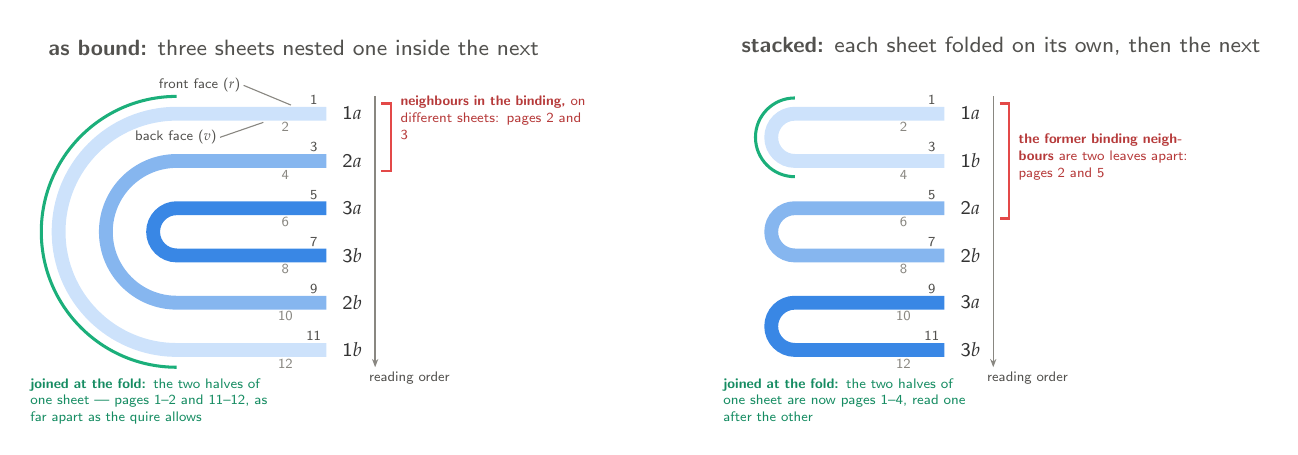
\begin{tikzpicture}[x=1cm,y=1cm,font=\sffamily\scriptsize]
\begin{scope}[shift={(1.75,0)}]
  \node[anchor=south west,font=\sffamily\footnotesize,color=ink2] at (-1.75,0.62) {\textbf{as bound:} three sheets nested one inside the next};
  \qnested{3}
  \qfacecallout
  \qfoldmark{-1.5}{1.72}
  \qfoldlabel{-1.9}{-3.32}{\textbf{joined at the fold:} the two halves of one sheet --- pages \mbox{1--2} and \mbox{11--12}, as far apart as the quire allows}
  \qreadarrow{6}
  \qbracket{leaf1a}{leaf2a}{nestedc}{0.15}{-0.05}{\textbf{neighbours in the binding,} on different sheets: pages 2 and 3}
\end{scope}
\begin{scope}[shift={(9.6,0)}]
  \node[anchor=south west,font=\sffamily\footnotesize,color=ink2] at (-0.8,0.62) {\textbf{stacked:} each sheet folded on its own, then the next};
  \qstacked{3}
  \qfoldmark{-0.3}{0.5}
  \qfoldlabel{-0.95}{-3.32}{\textbf{joined at the fold:} the two halves of one sheet are now pages 1--4, read one after the other}
  \qreadarrow{6}
  \qbracket{leaf1a}{leaf2a}{nestedc}{0.15}{-0.55}{\textbf{the former binding neighbours} are two leaves apart: pages 2 and 5}
\end{scope}
\end{tikzpicture}
\caption{The two arrangements being compared, drawn as a quire of three sheets seen from its top edge, spine at the left. Each folded sheet gives two leaves ($a$ above the fold, $b$ below); each leaf has a front face ($r$) and a back face ($v$); the small numbers are the order in which the faces are read---down the pile, front then back of each leaf. Left: nested as bound, so the two halves of a sheet lie at opposite ends of the quire and the pages that follow one another are mostly on different sheets. Right: the same sheets each folded on their own and laid one after the next (stacked), so a sheet's four pages are read together. The report's central test asks which pairs of leaves share rare material: the two halves of one sheet (aqua, joined at the fold) or leaves that are neighbours only in the binding (red bracket).}
\label{fig:es-schematic}
\end{figure}

\subsection*{Finding 1 --- The manuscript's rare words hardly cluster at all}

\begin{figure}[htbp]
\centering
\fig{fig_es_locality}
\caption{How much closer together than chance a text's rare words sit. For every word used exactly twice, the chance that its two uses fall within 100 words of each other, divided by the same chance under random placement. Prose clusters 13--51 times more than chance; the manuscript 3.8--3.9 times, less than rhymed verse; either Currier language on its own, less still. (\cref{sec:baseline}, \cref{tab:locality}.)}
\label{fig:es-locality}
\end{figure}

In known prose a twice-used word's two occurrences fall within 100 words of each other 13 to 51 times more often than chance; in the manuscript, under four times (\cref{fig:es-locality}). Against 148 windows of known text cut to the manuscript's length, the manuscript sits at the extreme low edge, with only Tasso and Dante below it; the pattern is the same for words used three, four or five times, and in both of the manuscript's ``languages'' (Currier A and B). Its rare words cluster like the rare rhyme-words of narrative verse, not like the topic words of prose.

\emph{What this means.} Two things. First, every test of order in this report has to find its signal in a text with about a tenth of the locality of the control texts, so the tests are weak, and where a result is null that is the expected outcome rather than evidence of absence. Second, this is a property of the text itself, whatever it is: its rare ``words'' do not behave as topic words do.

\subsection*{Finding 2 --- The two halves of a sheet belong together}

\begin{figure}[htbp]
\centering
\fig{fig_es_leaftest}
\caption{The leaf-pair test. Positive values: the two halves of one sheet share more rare material than pages that follow one another in the binding but lie on different sheets; negative: the reverse. The washes show what six real texts give when written onto the manuscript's own pages sheet by sheet (aqua) and in the binding order (red). (\cref{sec:leaf}, \cref{tab:leaf}.)}
\label{fig:es-leaftest}
\end{figure}

Despite the weak signal, the two halves of a physical sheet share rare material more than the pages that are neighbours only in the binding do---and the binding-neighbours share \emph{less} than random pages of the same quire (\cref{fig:es-leaftest}). On rare words the excess is 2.4--2.5 standard deviations above chance; on rare seven-glyph strings, an independent unit run as the pre-stated check, it is 4 to 5. The six control texts settle what that size means: written sheet by sheet they land in the same band as the manuscript, written in the binding order they land far on the other side, on all 36 of 36 comparisons each way. Two objections were tested. The scribes' hands run by sheet (97\,\% of sheet halves are in one hand), so a scribe's private spelling habits could mimic the effect: holding the hand fixed in the comparison leaves the glyph-string result unchanged. And an excess this large might arise by accident: in 5\,000 random re-placements of the pages it never did, on either transcription. One caution belongs here: the test on words used exactly twice was null, the pooled word statistic was chosen after that, and the glyph-string test was then run as the check; the glyph-string number is the one to quote.

\emph{What this means.} The text on one sheet is a unit. What this does \emph{not} decide is whether the sheet was the unit of \emph{reading} (Davis's proposal) or the unit of \emph{work}---one scribe, one sitting, one subject per sheet, with the nested reading order still intended. Every statistic in this report responds identically to the two.

\subsection*{Finding 3 --- No other way of gathering the sheets fits as well}

\begin{figure}[htbp]
\centering
\fig{fig_es_nesting}
\caption{Every way of gathering the six sheets of quire T, 23\,040 patterns in all. (a)~The best fit obtainable when the sheets are gathered as one nested block (the binding among them) up to six blocks (every sheet read whole): the fit improves at every step toward reading sheets whole. (b)~Where three arrangements rank among the 23\,040: the best stacked order, the best fully nested order and the binding as it is. (\cref{sec:nesting}, \cref{tab:nesting}.)}
\label{fig:es-nesting}
\end{figure}

Finding 2 compared the sheets read whole with one nested arrangement, the binding. Perhaps a different nesting, or two smaller gatherings placed one after another, would explain the text as well. For the six-sheet quire T every such pattern was scored, 23\,040 in all (\cref{fig:es-nesting}). The fit improves at every step from ``one nested block'' toward ``every sheet read whole''; the best fully nested arrangement ranks between 5\,007th and 10\,535th, the binding as it is between 13\,942nd and 22\,405th, and no pattern with two or three nested groups ever wins. The same holds, with smaller candidate sets and coarser odds, in the other four quires tested.

\emph{What this means.} The property the text rewards is exactly the one every stacked order has, a sheet's four pages kept together, and the comparison in Finding 2 was not a straw man: the binding is not merely worse than the best alternative, it is among the worst of all arrangements.

\subsection*{Finding 4 --- Inside quire T the sheets have a preferred order}

\begin{figure}[htbp]
\centering
\fig{fig_es_quireT}
\caption{Which sheet follows which in quire T (the ``stars'' quire, f103--f116, six sheets). (a)~All 720 orders of the six sheets scored by how close together rare glyph strings fall; the grey histogram is where the \emph{best} of 720 lands when the pages' contents are shuffled, which is the bar the real winner must clear. (b)~The sheets as bound and in the order the text prefers; the direction of reading along the chain is not established. (\cref{sec:seriation}, \cref{tab:quires}.)}
\label{fig:es-quireT}
\end{figure}

If a sheet is a unit, the sharing between sheets can say which sheet followed which. For the six sheets of quire T there are 720 orders; one of them, \order{1-6-5-4-2-3} (outermost sheet first, then the innermost, then outward), is chosen by 31 of 32 combinations of text unit, cost function and transcription (\cref{fig:es-quireT}). It fits four standard deviations better than the average order, where the best of 720 orders on shuffled page contents sits near three; against those shuffles its odds are at most 1 in 50 on every test, and the size of the sheets alone cannot produce it. The current bound order lies in the bottom half. Quire C, a herbal quire in the other Currier language and another hand, settles the same way on \order{1-4-3-2} on 30 of 32 tests; quire M is consistent with one family of orders; the two smallest herbal quires (1\,000--1\,500 words) tell nothing. In each of T, C and M the outermost sheet neighbours the innermost.

\emph{What this means.} Within at least one quire the text remembers an order of its sheets, and it is not the bound order. What it does not give is the \emph{direction} of reading along the chain: the gap between the winning order and its reversal is no larger than selection alone produces on shuffled pages, and there is no time arrow inside a burst of rare words to calibrate on (prose bursts are symmetric to within a per cent). Nor can the order be attributed to reading rather than to working sheet by sheet, for the reason given under Finding 2.

\subsection*{What the report establishes, and what it does not}

\begin{establishes}
\begin{itemize}
\item \textbf{The sheet is a unit of the text.} The two halves of a physical sheet share rare material more than pages that are neighbours only in the binding, on words and on glyph strings, in both transcriptions, with quire, language and scribal hand held fixed; real texts reproduce this only when written sheet by sheet (Finding 2).
\item \textbf{The binding as it is fits the text worse than almost any other arrangement of the same sheets,} and nothing but reading the sheets whole fits as well (Finding 3).
\item \textbf{Quire T has a recoverable sheet order,} \order{1-6-5-4-2-3}, replicated in shape by quire C (Finding 4).
\item \textbf{The manuscript's rare words carry about a tenth of the locality of prose} (Finding 1), which is why the effects above are small in absolute terms: three quarters of twice-used words span more than one quire, and no re-ordering of the manuscript's 52 sheets makes its rare words cluster like those of prose.
\end{itemize}
\end{establishes}

\begin{notestablished}
\begin{itemize}
\item \textbf{That the manuscript was meant to be \emph{read} sheet by sheet.} ``Written sheet by sheet as a unit of work, intended to be read nested'' produces every observation above. Text position cannot separate the two; production evidence (ink, ruling, the sequence of drawings) could.
\item \textbf{The direction of reading} along any chain of sheets.
\item \textbf{Which sheets or quires of the whole manuscript are out of place.} Five quires were seriated; the mixed-language quires, the large foldouts and the codicological literature's specific proposals were not tested.
\item \textbf{Anything about the language or a decipherment.} This is a side study; no solver or verdict of the main project depends on it, and the stacked order does not change the solver's inputs.
\end{itemize}
\end{notestablished}

\begin{table}[H]
\centering\small
\caption{Reading guide: the claims, how strong the evidence is, and where to find it.}
\label{tab:es-guide}
\renewcommand{\arraystretch}{1.15}
\begin{tabular}{@{}L{6.1cm}cL{5.9cm}c@{}}
\toprule
claim & strength & basis & where\\
\midrule
rare words cluster at $\approx$1/10 of prose & \esS & 148 known windows of equal length; both transcriptions & \cref{sec:baseline}\\
sheet halves share more than binding neighbours & \esS & $+3$ to $+5$ sd on glyph strings; 0/5\,000 random placements; 36/36 controls each way; hand-controlled & \cref{sec:leaf}\\
the effect is small in mass; no global re-ordering helps & \esS & rare words not contained by sheet; optimiser gains only its noise ceiling & \cref{sec:isnot}\\
every other gathering of the sheets loses to reading them whole & \esS\,/\,\esM & decisive in quire T (23\,040 patterns); coarser in M and the four-sheet quires & \cref{sec:nesting}\\
quire T order \order{1-6-5-4-2-3} & \esS & 31/32 tests; odds $\le$ 1 in 50 vs shuffled pages on every test; geometry excluded & \cref{sec:seriation}\\
quire C order \order{1-4-3-2} & \esM & 30/32 tests, but only 24 candidates, so the odds are coarse & \cref{sec:seriation}\\
quire M order family & \esW & consistent across units; words weak & \cref{sec:seriation}\\
quires A and B & \esN & too little text; no information & \cref{sec:seriation}\\
reading direction along a chain & \esN & gap to the reversal is what selection alone gives; no time arrow in bursts & \cref{sec:direction}\\
reading unit vs.\ working unit & \esX & not testable from text position & \cref{sec:discussion}\\
\bottomrule
\end{tabular}

\smallskip
{\footnotesize \esS\ strong \quad \esM\ moderate \quad \esW\ weak \quad \esN\ null / not established \quad \esX\ outside what the method can test}
\end{table}
\setcounter{figure}{0}\setcounter{table}{0}
\renewcommand{\thefigure}{\arabic{figure}}\renewcommand{\thetable}{\arabic{table}}
\clearpage

%=====================================================================
\section{Question and codicological setting}
\label{sec:question}

A bifolium---one \emph{sheet}---is folded once into two \emph{leaves} $a$ and $b$, giving four \emph{pages} $a^r, a^v, b^r, b^v$. A quire of $S$ sheets nests them: sheet~1 is outermost, sheet~$S$ innermost. Read as bound, the page sequence is
\begin{equation}
1a^r,\,1a^v,\;2a^r,\,2a^v,\;\dots,\;Sa^r,\,Sa^v,\;Sb^r,\,Sb^v,\;\dots,\;2b^r,\,2b^v,\;1b^r,\,1b^v ,
\label{eq:nested}
\end{equation}
so the two leaves of an outer sheet are far apart and consecutive leaves mostly belong to different sheets. Read \emph{stacked}, each sheet is read whole,
\begin{equation}
1a^r,\,1a^v,\,1b^r,\,1b^v,\;\;2a^r,\,2a^v,\,2b^r,\,2b^v,\;\;\dots
\label{eq:stacked}
\end{equation}
and the two leaves of a sheet are always adjacent (\cref{fig:codicology}). Two kinds of leaf pair therefore discriminate the arrangements: \emph{conjugate} leaves (the two leaves of one sheet, adjacent only under stacked reading) and \emph{nested-adjacent} leaves (consecutive in the binding but on different sheets, adjacent only under nested reading).

If a text was written continuously, words and phrases that belong to one passage sit close together \emph{in the writing order}. A rare word's recurrences are the cleanest carrier of that locality: a topic word used twice in 38\,000 words is used twice in the same passage. So the question ``was the text written in the nested order or the stacked order?'' becomes ``do conjugate leaves or nested-adjacent leaves share more rare material than chance?''---a question with a permutation null and known-text controls. Two further questions follow once the first is answered: whether the sheet sharing can \emph{order} the sheets of a quire (seriation), and whether it can give the \emph{direction} of reading along that order.

\paragraph{Provenance of the proposal, and a prior attempt.} The stacked-bifolia proposal is, to our knowledge, not in print. Davis put it forward once, in a public lecture,\footnote{Recorded lecture, online video (c.\,2023--24); the link will be added to this report once retrieved. \emph{[URL pending.]}} and said there that a colleague at the University of Malta was trying to test it against the text with latent semantic analysis (LSA)---that is, whether the topical similarity of pages favours the stacked over the nested sequence. We have found no journal or preprint account of that analysis, so its statistic, its controls and its outcome are unknown to us, and nothing below builds on it. The present study is therefore not the first attempt to look for the arrangement in the text but a second one, made independently and with a different instrument: not topic vectors over whole pages but the positions of individual rare types, a permutation null that holds quire, Currier language and scribal hand fixed, and six known texts written onto the manuscript's own page slots as positive and negative controls. If the LSA result becomes available, the point at which the two approaches should agree is the sign of the conjugate-versus-nested contrast of \cref{sec:leaf}; they need not agree on the within-quire seriation of \cref{sec:seriation}, which uses a finer unit than any page-level topic model.

\begin{figure}[tbp]
\centering
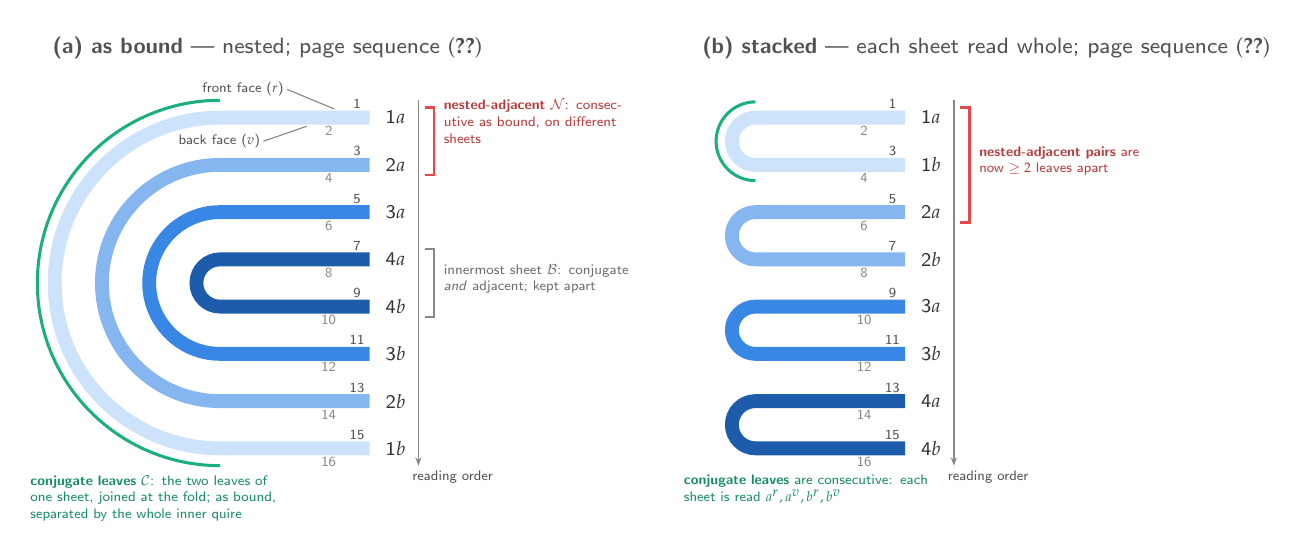
\begin{tikzpicture}[x=1cm,y=1cm,font=\sffamily\scriptsize]
\begin{scope}[shift={(2.25,0)}]
  \node[anchor=south west,font=\sffamily\footnotesize,color=ink2] at (-2.25,0.62) {\textbf{(a) as bound} --- nested; page sequence \eqref{eq:nested}};
  \qnested{4}
  \qfacecallout
  \qfoldmark{-2.1}{2.32}
  \qfoldlabel{-2.45}{-4.5}{\textbf{conjugate leaves $\mathcal{C}$}: the two leaves of one sheet, joined at the fold; as bound, separated by the whole inner quire}
  \qreadarrow{8}
  \qbracket{leaf1a}{leaf2a}{nestedc}{0.15}{-0.05}{\textbf{nested-adjacent $\mathcal{N}$}: consecutive as bound, on different sheets}
  \qbracket{leaf4a}{leaf4b}{muted}{0.15}{-0.25}{innermost sheet $\mathcal{B}$: conjugate \emph{and} adjacent; kept apart}
\end{scope}
\begin{scope}[shift={(9.05,0)}]
  \node[anchor=south west,font=\sffamily\footnotesize,color=ink2] at (-0.8,0.62) {\textbf{(b) stacked} --- each sheet read whole; page sequence \eqref{eq:stacked}};
  \qstacked{4}
  \qfoldmark{-0.3}{0.5}
  \qfoldlabel{-0.95}{-4.5}{\textbf{conjugate leaves} are consecutive: each sheet is read $a^r, a^v, b^r, b^v$}
  \qreadarrow{8}
  \qbracket{leaf1a}{leaf2a}{nestedc}{0.15}{-0.55}{\textbf{nested-adjacent pairs} are now $\ge 2$ leaves apart}
\end{scope}
\end{tikzpicture}
\caption{Nested versus stacked reading of a four-sheet quire, seen from its top edge with the spine at the left. Leaf $a$ of each sheet lies above its fold and leaf $b$ below; the numbers give the reading position of each leaf's front ($r$) and back ($v$) face, read down the pile. (a)~The binding, \cref{eq:nested}: conjugate leaves $\mathcal{C}$---the two leaves of one sheet, joined at the fold (aqua)---are separated by the whole inner quire, while the leaves that follow one another lie on different sheets (nested-adjacent pairs $\mathcal{N}$, red); the innermost sheet's two leaves are both at once ($\mathcal{B}$) and are excluded from the statistic. (b)~The stacked order, \cref{eq:stacked}: each sheet is read $a^r,a^v,b^r,b^v$, so conjugate leaves are consecutive and the former nested-adjacent pairs are at least two leaves apart. A text written in one order and bound in the other leaves its rare-word locality on the ``wrong'' leaf pairs.}
\label{fig:codicology}
\end{figure}

%=====================================================================
\section{Data, units and notation}
\label{sec:data}

\paragraph{Streams.} Both public EVA transcriptions are used throughout: Takahashi (\IT) and the Reference transcription (\RF). Tokens containing an uncertain glyph are dropped whole; extended-EVA codes and ligature braces are kept as part of the word type. In folio order the streams hold 37\,759 (\IT) / 38\,463 (\RF) tokens on 225 / 227 pages, mean 168 tokens per page; 896 / 997 doubleton types and 5\,527 / 6\,685 hapax types. Page headers supply quire, bifolium, Currier language ($A$/$B$), section and scribal hand (Davis's five scribes). \src{1}

\paragraph{Rare types.} A \emph{type} is a word type or, for the sub-word analyses, a character $n$-gram ($n=4$--8) over the space-stripped page text, with extended-EVA codes as single symbols. A type $t$ with occurrence set $O_t$ is \emph{rare} when $k_t=|O_t|\in[2,10]$; $k_t=2$ is a doubleton. The variant \emph{cross} keeps only $n$-grams that straddle a word boundary, so that they are fragments of word \emph{pairs} rather than of single rare words. \src{7}

\paragraph{Known texts.} Latin (Isidore, Seneca \emph{NQ}, Pliny, Macer, Gordon, Hyginus, Bacon), German (Bullinger, Staden, Promptuarium, Küchenmeisterei) and Italian (Decameron, Principe, Commedia, Orlando Furioso) texts from the project corpus, cut into windows of 37\,759 tokens and pseudo-pages of 168 tokens; for the corpus sweep, every corpus document of $\ge 37\,759$ words (148 windows: German 113, Latin 25, Italian 10). \src{1, 9}

\paragraph{Notation.} Pages are slots $p=1..P$ with contents $c_p$ (a bag of typed occurrences) and token length $L_p$. $q(p)$, $\lambda(p)$, $h(p)$, $s(p)$ and $\ell(p)$ denote quire, Currier language, hand, sheet and leaf. An \emph{occurrence pair} is $(i,j)$, $i<j$, two occurrences of the same rare type on different pages. For a page order $\sigma$, $\mathrm{pos}_\sigma(i)$ is the token index of occurrence $i$ and $d_\sigma(i,j)=|\mathrm{pos}_\sigma(i)-\mathrm{pos}_\sigma(j)|$.

\paragraph{Empirical $p$-values.} Every $p$ quoted below is a Monte-Carlo tail with the add-one convention,
\begin{equation}
\pv=\frac{\#\{\text{null draws at least as extreme as observed}\}+1}{n_{\text{draws}}+1},
\label{eq:pemp}
\end{equation}
so with 200 draws the floor is $1/201\approx 0.005$ and with 5\,000 draws $\approx 2\times10^{-4}$. A $z$ is $(\text{obs}-\bar{x}_{\text{null}})/s_{\text{null}}$; where the null's shape matters it was checked directly (\cref{sec:nullshape}).

%=====================================================================
\section{How local is the manuscript's rare material?}
\label{sec:baseline}

The power of every order test is set by how tightly a text's rare types cluster in its writing order. For a type with $k$ occurrences at positions $x_1<\dots<x_k$ in a stream of $N$ tokens, the consecutive gaps $g_m=x_{m+1}-x_m$ are compared with their distribution under uniform placement of $k$ points on $N$ (exact for $k=2$; 200\,000 Monte-Carlo draws for $k\ge3$). The locality ratio at scale $G$ is
\begin{equation}
r_G=\frac{\Pr(g\le G)}{\Pr_{\text{unif}}(g\le G)} .
\label{eq:rG}
\end{equation}

\begin{table}[t]
\centering\small
\caption{Rare-type locality $r_{100}$ by frequency class $k$ (in brackets: percentage of types with all occurrences on one page). Manuscript rows are the whole stream; Currier $A$ and $B$ alone are 11\,k and 23--24\,k tokens. \src{2, 6.1}}
\label{tab:locality}
\footnotesize\setlength{\tabcolsep}{4pt}
\begin{tabular}{@{}lcccc@{}}
\toprule
text & $k=2$ & $k=3$ & $k=4$ & $k=5$\\
\midrule
VMS \IT\ (types 896 / 399 / 216 / 145) & 3.8 (2.9\,\%) & 3.3 (0.3\,\%) & 3.5 (0\,\%) & 4.5 (0\,\%)\\
VMS \RF\ (997 / 413 / 250 / 157) & 3.9 (2.3\,\%) & 3.7 (0.2\,\%) & 5.0 (0.8\,\%) & 4.4 (0.6\,\%)\\
Currier $A$ alone (\IT\ / \RF) & 2.4 / 3.1 & 2.7 / 2.9 & 2.9 / 3.2 & 3.2 / 2.6\\
Currier $B$ alone & 2.6 / 3.2 & 3.3 / 3.0 & 2.9 / 3.0 & 3.0 / 1.9\\
\addlinespace
Isidore (Latin prose) & 51 (23\,\%) & 32 (7.0\,\%) & 23 (2.2\,\%) & 18 (0.5\,\%)\\
Pliny (Latin prose) & 21 (10\,\%) & 19 (3.5\,\%) & 12 (0.3\,\%) & 12 (1.3\,\%)\\
Seneca \emph{NQ} (Latin prose) & 13 (5.4\,\%) & 9.5 (1.9\,\%) & 8.6 (0.3\,\%) & 6.0 (0\,\%)\\
Bullinger, Staden (German prose) & 23--26 (11\,\%) & 16--17 (3\,\%) & 14--15 (0.5--1.3\,\%) & 9--11 (0.6--0.8\,\%)\\
Decameron (Italian prose) & 13 (6.0\,\%) & 13 (1.3\,\%) & 7.1 (0.4\,\%) & 7.9 (0\,\%)\\
Commedia, Orlando Furioso (verse) & 6.6--8.4 (3.8\,\%) & 4.4--4.7 (0--0.6\,\%) & 4.4--5.4 (0\,\%) & 2.4--3.9 (0\,\%)\\
\bottomrule
\end{tabular}
\end{table}

\Cref{tab:locality} and \cref{fig:locality} give the result. In prose a word used twice in 38\,k tokens is a topic word and its two uses sit in the same passage: $r_{100}=12$--50, with 5--23\,\% of doubletons on one page. The manuscript's doubletons show a tenth of that ($r_{100}=3.8$--3.9, 2--3\,\% same page), below even Italian narrative verse (6.8--10, 4\,\%), whose rare forms are scattered by rhyme and metre; the excess within 10 tokens ($r_{10}=4$--8) is the known line-level near-repeat phenomenon. The picture does not change with $k$: at every frequency class the manuscript clusters like rhymed verse, not like prose, in both Currier languages. \src{2, 6.1}

The corpus sweep places the manuscript against 148 known windows on the pooled $k\in[2,5]$ statistic: known $r_{100}$ runs from 3.39 (5th percentile 4.66, median 12.9) to 34.0; \IT\ scores 3.89 (2.5th percentile, log-$z$ $-2.3$; below it only Tasso's \emph{Gerusalemme liberata}), \RF\ 4.38 (3.8th percentile, log-$z$ $-2.1$; below it Tasso and Dante).\footnote{The recorded percentiles were computed on the sweep log's 158 windows, which include the ten Italian raw-text documents twice; on the 148 de-duplicated windows they are 1.4\,\% (\IT) and 2.0\,\% (\RF). Either way the manuscript sits at the extreme low edge of the corpus.} Currier $A$ or $B$ alone score 2.8--2.9, below every known window. The whole-manuscript stream mixes languages and sections, which \emph{adds} clustering, so these are upper bounds on the within-section locality. \src{9}

This agrees with the two published scales: section-level vocabulary information (Montemurro \& Zanette) is present---adjacent-page sharing is $z=6$--7 under a global page shuffle and mostly removed by permuting only within section \src{3}---while at passage scale rare recurrences are nearly memoryless (Reddy \& Knight; Schinner). Whatever a manuscript ``word'' is, its rare recurrences carry very little topical locality; every test below has to find an order signal in a text with roughly one tenth of the locality of the controls.

\begin{figure}[tbp]
\centering
\fig{fig_locality_baseline}
\caption{Rare-type locality. (a)~$r_{100}$ by frequency class $k$ for the manuscript (whole stream and Currier $A$/$B$ alone) against known prose and verse (\cref{tab:locality}). (b)~Corpus sweep: 148 known 37\,759-token windows on the pooled $k\in[2,5]$ statistic, with the two manuscript transcriptions marked at their percentiles among these 148 windows (the recorded 2.5\,\% / 3.8\,\% were on the sweep log\textquoteright s 158-window count; see the footnote in the text). \src{6.1, 9}}
\label{fig:locality}
\end{figure}

%=====================================================================
\section{The leaf-pair test}
\label{sec:leaf}

\subsection{Statistic and null}

Let $\mathcal{P}$ be the set of occurrence pairs of rare types whose two members lie on different leaves of the \emph{same quire}. Each pair is classified by the relation between its two leaves:
\begin{itemize}
\item[$\mathcal{C}$] conjugate: $s(i)=s(j)$, $\ell(i)\neq\ell(j)$---the two leaves of one sheet;
\item[$\mathcal{N}$] nested-adjacent: the leaves are consecutive in the binding and $s(i)\neq s(j)$;
\item[$\mathcal{B}$] the innermost sheet, whose two leaves are both conjugate and nested-adjacent (kept apart);
\item[$\mathcal{O}$] every other same-quire leaf pair.
\end{itemize}
The statistic is the difference of the two discriminating counts,
\begin{equation}
\Dstat=n_{\mathcal{C}}-n_{\mathcal{N}},\qquad n_X=\#\{(i,j)\in\mathcal{P}:\ (i,j)\in X\}.
\label{eq:D}
\end{equation}
The null permutes page \emph{contents} among page \emph{slots} within groups $g(p)=(q(p),\lambda(p))$---quire and Currier language---or, for the hand control, $g(p)=(q(p),\lambda(p),h(p))$. A permutation $\pi$ moves whole pages, so every page keeps its own rare-word load and its own within-page clumping; only which physical slot a page occupies is randomised. $\Dstat_\pi$ is recomputed per draw ($2\,000$ draws; $5\,000$ for the tail study, \cref{sec:tail}), giving $z_{\Dstat}$ and \cref{eq:pemp}. Because the innermost sheet is excluded from both $\mathcal{C}$ and $\mathcal{N}$ and every quire with a single sheet contributes nothing, $\Dstat$ is driven by quires with $\ge 2$ sheets.

Under a text written in the nested order \cref{eq:nested}, passage locality lands on $\mathcal{N}$ pairs and $\Dstat<0$; under a text written in the stacked order \cref{eq:stacked} it lands on $\mathcal{C}$ pairs and $\Dstat>0$; under evenly spread rare material $\Dstat\approx0$.

\subsection{Power controls}

The magnitude of $\Dstat$ under either hypothesis depends on the text's locality (\cref{sec:baseline}), so it is calibrated with known texts laid onto the \emph{manuscript's own page slots}: the same tokens per page (symbols per page for $n$-grams), the same quire and sheet structure. Each text is written either in the nested order or in the stacked order, then bound nested and analysed identically. Six texts were used (Isidore, Seneca \emph{NQ}, Bullinger, Decameron, Commedia, Orlando Furioso), covering 3--13$\times$ the manuscript's locality.

\subsection{Results}

\begin{table}[t]
\centering\small
\caption{The leaf-pair statistic $\Dstat=n_{\mathcal C}-n_{\mathcal N}$ (\cref{eq:D}) on the manuscript, as $z$ against the within-quire-and-language page-permutation null, and the range of $z_{\Dstat}$ the six control texts give on the same page slots when written nested or stacked. Word rows pool types with the stated $k$; $n$-gram rows are $k\in[2,10]$. \src{4, 6.2, 7.1, 7.2}}
\label{tab:leaf}
\begin{tabular}{@{}llccccc@{}}
\toprule
& & \multicolumn{2}{c}{manuscript $z_{\Dstat}$} & & \multicolumn{2}{c}{controls $z_{\Dstat}$ (six texts)}\\
\cmidrule(lr){3-4}\cmidrule(lr){6-7}
unit & pairs (\IT/\RF) & \IT & \RF & & written nested & written stacked\\
\midrule
words, $k=2$ & 896 / 997 & $+0.7$ & $-0.1$ & & $-1.8$ to $-4.0$\,$^\dagger$ & $+0.2$ to $+3.9$\,$^\dagger$\\
words, $k\in[2,5]$ & 4\,839 / 5\,306 & $+2.5$ & $+1.8$ & & $-0.8$ to $-7.1$ & $+0.9$ to $+3.6$\\
words, $k\in[2,10]$ & 13\,665 / 14\,625 & $+2.4$ & $+2.5$ & & $-2.0$ to $-7.3$ & $+1.5$ to $+4.7$\\
\addlinespace
$n$-grams $n=4$, all & 33\,k / 37\,k & $+2.6$ & $+1.2$ & & --- & ---\\
$n=5$, all & 74\,k / 81\,k & $+3.4$ & $+2.8$ & & $-2.2$ to $-6.3$ & $+1.1$ to $+4.7$\\
$n=6$, all & 113\,k / 119\,k & $+3.3$ & $+3.5$ & & $-3.4$ to $-7.6$ & $+1.7$ to $+4.5$\\
$n=7$, all & 119\,k / 118\,k & $+4.1$ & $+4.4$ & & $-3.7$ to $-7.8$ & $+1.9$ to $+4.5$\\
$n=8$, all & 98\,k / 92\,k & $+4.7$ & $+4.8$ & & --- & ---\\
\addlinespace
$n=5$, cross & & $+3.1$ & $+2.3$ & & $-1.7$ to $-7.0$ & $+1.3$ to $+4.7$\\
$n=6$, cross & & $+3.2$ & $+3.5$ & & $-2.4$ to $-7.2$ & $+1.6$ to $+4.9$\\
$n=7$, cross & & $+3.7$ & $+4.2$ & & $-2.4$ to $-7.3$ & $+1.4$ to $+4.3$\\
$n=8$, cross & & $+4.4$ & $+5.2$ & & --- & ---\\
\bottomrule
\multicolumn{7}{@{}l@{}}{\footnotesize $^\dagger$ five texts (no Commedia), 500 shuffles; verse written stacked is indistinguishable from the null at $k=2$.}
\end{tabular}
\end{table}

\paragraph{Doubletons alone cannot tell.} With the 896 / 997 doubletons, $\Dstat$ is $-9$ against a null of $-13.3\pm6.3$ (\IT, $z=+0.7$) and $-14$ against $-13.4\pm6.6$ (\RF, $z=-0.1$). The controls show why: even texts with 3--13$\times$ the manuscript's locality separate the two hypotheses by only 2--7\,sd at $k=2$, and stacked-written verse is indistinguishable from the null. The manuscript's value lies above every nested-written control and inside the stacked-written band, but its expected magnitude under \emph{either} hypothesis is smaller than any control's. \src{4}

\paragraph{Pooling rare types.} Pooling all occurrence pairs of types with $k\in[2,10]$ raises the pair count to 13.7\,k / 14.6\,k and puts the manuscript at $z_{\Dstat}=+2.4/+2.5$---inside the stacked-written band ($+0.9$ to $+4.7$) and outside the nested-written band ($-0.8$ to $-7.3$, all six texts, both pool sizes). Both components move: conjugate leaves share \emph{more} than random same-quire leaves ($z=+2.2/+2.3$) and nested-adjacent leaves share \emph{less} ($z=-1.8/-1.8$). The excess is spread over quires A (herbal, Currier $A$), T (stars, $B$), H and M and absent from herbal quires B--G; Currier $B$ pages alone give $+1.8/+1.9$, Currier $A$ pages alone $+0.3/+0.7$. This pooled statistic was chosen \emph{after} the $k=2$ test came back null, so its nominal one-sided $p\approx0.01$ is not pre-registered. \src{6.2}

\paragraph{Glyph $n$-grams: the pre-stated confirmation.} An independent unit was run as the check of the pooled-word hypothesis: character $n$-grams, $n=4$--8, $k\in[2,10]$, with the cross variant to exclude fragments of single rare words. The excess grows with $n$ from $+2.6/+1.2$ at $n=4$ to $+4.7/+4.8$ at $n=8$ (cross $+4.4/+5.2$); doubleton $n$-grams alone give $+4.5/+3.4$ at $n=7$. On the controls, all 36 nested-written cells (six texts $\times$ $n=5,6,7$ $\times$ all/cross) are negative ($-1.7$ to $-7.8$) and all 36 stacked-written cells positive ($+1.1$ to $+4.9$); the manuscript's $+3$ to $+5$ sits in the upper part of the stacked-written band (\cref{fig:leaftest}, \cref{fig:leafcontrols}). \src{7.1, 7.2}

\begin{figure}[tbp]
\centering
\fig{fig_leaf_test}
\caption{The leaf-pair statistic on the manuscript. (a)~$z_{\Dstat}$ by unit (words at three pool sizes; $n$-grams $n=4$--8, all and boundary-straddling) for both transcriptions, with the control bands: the range of $z_{\Dstat}$ six known texts give on the same page slots when written nested (red) or stacked (aqua); hollow markers are the hand-controlled null. (b)~The two components, conjugate and nested-adjacent, separately. \src{4, 6.2, 7}}
\label{fig:leaftest}
\end{figure}

\begin{figure}[tbp]
\centering
\fig{fig_leaf_test_controls}
\caption{Power controls, per text: $z_{\Dstat}$ when the text is written in the nested order (red) and in the stacked order (aqua) onto the manuscript's page slots, for words $k\in[2,10]$ and $n$-grams $n=5,6,7$. Every nested-written cell is negative and every stacked-written cell positive; the manuscript's values are the reference lines. \src{6.2, 7.2}}
\label{fig:leafcontrols}
\end{figure}

\subsection{Scribal hand}
\label{sec:hand}

Conjugate leaves are in the same hand (and language) for 97\,\% of page pairs (138/142 \IT, 146/152 \RF); nested-adjacent leaves only 70\,\% (203/290, 203/292) and other same-quire pairs 73--75\,\%. The hands run by sheet---itself a codicological observation consistent with sheets being the working unit---so a hand-specific spelling habit could make conjugate leaves share rare $n$-grams for reasons unrelated to reading order. Restricting the null to permutations within quire, language \emph{and} hand (28 / 30 groups) removes that route (\cref{tab:hand}): the $n$-gram result is unchanged and the word result drops by about a third but keeps its sign. \src{7.3}

\begin{table}[t]
\centering\small
\caption{Hand control: $z_{\Dstat}$ (\IT\ / \RF) when page contents are permuted within quire and language, and within quire, language and hand. \src{7.3}}
\label{tab:hand}
\begin{tabular}{@{}lcc@{}}
\toprule
unit ($k\in[2,10]$) & null: quire + language & null: quire + language + hand\\
\midrule
words & $+2.4$ / $+2.5$ & $+1.7$ / $+2.0$\\
$n=6$ all ; cross & $+3.4$ / $+3.3$ ; $+2.9$ / $+3.2$ & $+3.5$ / $+3.7$ ; $+3.0$ / $+3.6$\\
$n=7$ all ; cross & $+3.9$ / $+4.1$ ; $+3.6$ / $+4.1$ & $+4.0$ / $+4.2$ ; $+3.6$ / $+4.2$\\
\bottomrule
\end{tabular}
\end{table}

\subsection{How often does even spreading produce the excess?}
\label{sec:tail}

The $z$ values assume nothing about the null's shape, but a tail of a few in $10^{5}$ should be counted, not extrapolated. \Cref{tab:tail} gives, for 5\,000 draws per cell, the number of null draws reaching the observed $\Dstat$ under two readings of ``evenly spread'': \emph{perm}, the page-content permutation above (the conservative reading, since page-level clumping stays in the variance), and \emph{uniform}, every occurrence of a rare type landing independently on a page of its language with probability proportional to page length. \src{12}

\begin{table}[t]
\centering\small
\caption{Empirical tail of $\Dstat$: null draws (of 5\,000) reaching the observed value, \IT\ / \RF, with the normal-tail $p$ for the recorded $z$. Under the uniform null every $n$-gram cell is 0/5\,000 ($z=+3.6$ to $+8.2$) and the word cell 10 / 0. \src{12}}
\label{tab:tail}
\footnotesize\setlength{\tabcolsep}{4pt}
\begin{tabular}{@{}lcccccc@{}}
\toprule
& \multicolumn{3}{c}{perm within quire + language} & \multicolumn{3}{c}{perm within quire + language + hand}\\
\cmidrule(lr){2-4}\cmidrule(lr){5-7}
unit ($k\in[2,10]$) & draws $\ge$ obs & $z$ & normal tail & draws $\ge$ obs & $z$ & normal tail\\
\midrule
words & 54 / 26 & $+2.3$ / $+2.5$ & $1/90$ $\cdot$ $1/190$ & 157 / 57 & $+1.8$ / $+2.0$ & $1/30$ $\cdot$ $1/90$\\
$n=5$ & 1 / 14 & $+3.5$ / $+2.9$ & & 2 / 2 & $+3.5$ / $+3.3$ & \\
$n=6$ & 3 / 3 & $+3.5$ / $+3.5$ & $\approx1/1\,700$ & 5 / 1 & $+3.6$ / $+3.7$ & \\
$n=7$ & \textbf{0 / 0} & $+4.2$ / $+4.3$ & $\approx1/70\,000$ & \textbf{0 / 0} & $+4.1$ / $+4.3$ & \\
$n=8$ & \textbf{0 / 0} & $+4.6$ / $+5.0$ & $\approx1/500\,000$ & \textbf{0 / 0} & $+4.5$ / $+4.9$ & \\
\bottomrule
\end{tabular}
\end{table}

The word-level excess alone is a 1-in-30 to 1-in-200 event under even spreading---real but not decisive, and chosen after a null result. The $n$-gram excess, the pre-stated confirmation, never occurs in 5\,000 even-spread draws at $n\ge7$ on either transcription or either null; its normal-tail chance is of order $10^{-5}$--$10^{-6}$ per cell. The cells are not independent ($n$-grams of neighbouring $n$ overlap and the two transcriptions are one text), so the family is best counted as one test per transcription at $n=7$ or 8; even a twenty-fold multiplicity correction leaves it below $1/1\,000$ (\cref{fig:tail}).

\begin{figure}[tbp]
\centering
\fig[0.85\textwidth]{fig_leaf_test_tail}
\caption{Empirical tail of the leaf-pair excess: null draws out of 5\,000 reaching the observed $\Dstat$, by unit, null and transcription; zero counts are shown explicitly. \src{12}}
\label{fig:tail}
\end{figure}

\FloatBarrier
\begin{establishes}[unbreakable]
Text on the two leaves of one physical sheet shares its rare material more than text on leaves that are neighbours only in the binding, and the nested neighbours share \emph{less} than random same-quire leaves. Three units (words, within-word $n$-grams, boundary-straddling $n$-grams), two transcriptions and a null holding quire, Currier language and hand fixed agree; six real texts written in the binding order never show this (36/36 cells negative) and written sheet by sheet always do (36/36 positive) at the manuscript's magnitude. Under even spreading the $n\ge7$ excess is a $\lesssim10^{-4}$ event.
\end{establishes}

%=====================================================================
\section{What the sheet effect is and is not}
\label{sec:isnot}

\subsection{Rare types are not contained by sheet}

The sheet effect could mean that rare types are \emph{held} by one bifolium. They are not (\cref{tab:containment}, \cref{fig:containment}a). Three quarters of doubletons and over 90\,\% of the 3--5-times types span more than one quire; only 2--3\,\% of doubletons and $\approx$0--1\,\% of the rest fall within a single sheet. The \cref{sec:leaf} effect is a small excess in the roughly 20\,\% of pairs that fall within a quire (same-leaf 2.7\,\% vs 1.6\,\% expected; same-sheet 2.6\,\% vs 2.3\,\%). This is why the two re-ordering exercises below move the locality statistics so little: the material an order can act on is a fifth of the pairs. \src{11}

\begin{table}[t]
\centering\small
\caption{Where the occurrences of a rare type sit: percentage of types with all occurrences in the given unit, \IT\ / \RF\ (null in brackets: page contents shuffled within quire and language, 200 draws; same-page and $2^{+}$-quire columns are order-invariant under that null). \src{11}}
\label{tab:containment}
\footnotesize\setlength{\tabcolsep}{4pt}
\begin{tabular}{@{}rrccccc@{}}
\toprule
$k$ & types & same page & same leaf ($r+v$) & same sheet, both leaves & $2^{+}$ sheets, same quire & $2^{+}$ quires\\
\midrule
2 & 896 / 997 & 2.9 / 2.3 & 2.7 / 2.6 (1.6 / 1.8) & 2.6 / 2.8 (2.3 / 2.6) & 14.3 / 14.4 (15.6 / 15.5) & \textbf{77.6 / 77.8}\\
3 & 399 / 413 & 0.3 / 0.2 & 0.3 / 0.5 (0.2 / 0.1) & 1.0 / 0.2 (0.4 / 0.3) & 7.3 / 8.0 (8.0 / 8.4) & \textbf{91.2 / 91.0}\\
4 & 216 / 250 & 0.0 / 0.8 & 0.0 / 0.0 & 0.0 / 0.4 (0.1 / 0.1) & 7.4 / 6.8 (7.4 / 7.0) & \textbf{92.6 / 92.0}\\
5 & 145 / 157 & 0.0 / 0.6 & 0.0 / 0.0 & 0.0 / 0.6 (0.0 / 0.1) & 3.4 / 3.8 (3.4 / 4.3) & \textbf{96.6 / 94.9}\\
\bottomrule
\end{tabular}
\end{table}

\subsection{The stacked order does not change solver windows}

The decipherment programme's word-homophonic solver has a findability wall near 4 tokens per type and had rejected windowing at 1.8--2.0 tokens/type per 1\,024-token window. Re-reading the Currier $A$ and $B$ streams in the stacked order changes tokens/type in non-overlapping windows by $\le0.01$ (under 1\,\%) at $W\le1\,024$---occasionally detectable against the within-quire page-shuffle null ($+3.2$\,sd for $A$ at $W=512$ on \IT\ and $B$ at $W=1\,024$ on \RF)---and by nothing or slightly negatively at $W\ge2\,048$; every window stays at 1.5--3.0 tokens/type with 70--80\,\% hapax types (\cref{fig:containment}b). The order result opens no solver path. \src{8}

\begin{figure}[tbp]
\centering
\fig{fig_containment}
\caption{(a)~Containment of rare types by codicological unit, \cref{tab:containment}. (b)~Tokens per type in non-overlapping windows of the Currier $A$ and $B$ streams read nested versus stacked. \src{11, 8}}
\label{fig:containment}
\end{figure}

\subsection{No sheet order lifts the locality above the noise ceiling}
\label{sec:optimize}

If the sheets were misarranged, a better stacking order should raise the manuscript's rare-word locality toward the corpus. Simulated annealing (20\,000 steps) over sheet orders was run on \IT\ (52 sheets, single surviving leaves counted as sheets, every sheet read stacked) with objective $J(\sigma)=\sum_{(i,j)}\exp(-d_\sigma(i,j)/1000)$ over consecutive occurrences of types with $k\in[2,5]$, under four constraint levels---\emph{strict} (swaps only within the same Currier language, section and hand; 12 groups), \emph{topic} (language + section; 10), \emph{language} (3), \emph{free}---and reported as $r_{100}$ and $r_{1000}$ (\cref{eq:rG}), whose corpus percentiles are known from \cref{sec:baseline} ($r_{1000}$: 5th percentile 1.65, 25th 2.74, median 3.35). \src{10}

\begin{table}[t]
\centering\small
\caption{Sheet-order optimisation, orientation fixed: $r_{100}$ / $r_{1000}$ after annealing under each constraint level. The page-content-shuffled manuscript has no order information and shows the optimiser's noise ceiling; known texts written stacked and shuffled are returned to their true-order value. \src{10}}
\label{tab:optimize}
\footnotesize\setlength{\tabcolsep}{4pt}
\begin{tabular}{@{}llccccc@{}}
\toprule
start & stat. & init & strict & topic & language & free\\
\midrule
\multirow{2}{*}{manuscript, stacked order} & $r_{100}$ & 4.04 & 4.24 & 4.28 & 4.24 & 4.48\\
 & $r_{1000}$ & 2.09 & 2.40 & 2.45 & 2.50 & 2.62\\
\addlinespace
\multirow{2}{*}{manuscript, random sheet orders (3 starts)} & $r_{100}$ & 4.04 & 4.2 & 4.1--4.2 & 4.2--4.4 & 4.3--4.4\\
 & $r_{1000}$ & 2.09 & 2.42--2.45 & 2.43--2.47 & 2.42--2.51 & 2.58--2.68\\
\addlinespace
\multirow{2}{*}{manuscript, page contents shuffled first (3 draws)} & $r_{100}$ & 4.0--4.5 & 5.3--5.7 & 5.1--5.4 & 5.3--5.9 & 6.1--6.6\\
 & $r_{1000}$ & 1.89--1.97 & 2.32--2.54 & 2.37--2.59 & 2.51--2.83 & 2.67--3.00\\
\midrule
\multicolumn{7}{@{}l}{\emph{known texts written stacked, sheets shuffled; ``init'' column gives the true-order value}}\\
\multirow{2}{*}{Isidore} & $r_{100}$ & 29.3 & 29.2 & 29.3 & 29.2 & 29.2\\
 & $r_{1000}$ & 5.09 & 5.09 & 5.11 & 5.09 & 5.16\\
\multirow{2}{*}{Seneca \emph{NQ}} & $r_{100}$ & 8.69 & 8.64 & 8.69 & 8.59 & 8.77\\
 & $r_{1000}$ & 2.51 & 2.52 & 2.56 & 2.61 & 2.64\\
\multirow{2}{*}{Bullinger} & $r_{100}$ & 14.8 & 14.6 & 14.7 & 14.5 & 14.8\\
 & $r_{1000}$ & 3.36 & 3.46 & 3.46 & 3.50 & 3.55\\
\multirow{2}{*}{Decameron} & $r_{100}$ & 9.27 & 9.30 & 9.20 & 9.30 & 9.30\\
 & $r_{1000}$ & 2.81 & 2.95 & 2.94 & 3.07 & 3.16\\
\multirow{2}{*}{Orlando Furioso} & $r_{100}$ & 5.36 & 5.56 & 5.43 & 5.52 & 5.49\\
 & $r_{1000}$ & 1.96 & 2.07 & 2.10 & 2.21 & 2.21\\
\bottomrule
\end{tabular}
\end{table}

Four readings of \cref{tab:optimize} and \cref{fig:optimize}. (i)~Re-ordering the sheets under any constraint moves $r_{1000}$ from 2.09 to 2.4--2.6, but a manuscript whose page contents were first shuffled---so that no order information exists---is moved by the same optimiser to 2.3--3.0: the whole gain is what an optimiser extracts from noise on $\sim$5\,000 rare pairs. (ii)~Random sheet orders are optimised to the same values as the actual stacked order; the current order is not a special optimum. (iii)~Known texts written sheet by sheet and shuffled are put back to their true-order value plus 0.0--0.35 of over-fitting, so the method would recover a real order if one carried locality. (iv)~Even the over-fitted manuscript values stay at the bottom of the corpus ($r_{1000}$ 2.4--2.6 is below the 25th percentile), and $r_{100}$ barely moves because gaps under 100 tokens fall inside a sheet ($\approx$670 tokens). Allowing inverted folding ($b^v,b^r,a^r,a^v$) adds $\approx+0.05$ to both the manuscript and the noise runs. Sheet order is not what separates the manuscript's rare vocabulary from prose; the separation is within the sheet. \src{10}

\begin{figure}[tbp]
\centering
\fig{fig_order_optimize}
\caption{Sheet-order optimisation. $r_{1000}$ after annealing under each constraint level for the manuscript from its stacked order and from random sheet orders, for the page-content-shuffled manuscript (noise ceiling), and for five known texts recovering their true-order value; corpus percentiles as reference lines. \src{10}}
\label{fig:optimize}
\end{figure}

%=====================================================================
\section{Seriation within a quire}
\label{sec:seriation}

The leaf-pair test says the sheet is a unit. Can the rare material also say \emph{which sheet follows which}? For a quire of $S$ sheets there are $S!$ stacked orders (each sheet read $a^r,a^v,b^r,b^v$), plus the nested binding as one more candidate (\cref{sec:nesting} widens the set to every nesting pattern of the sheets). Quires that are one language, one hand and one section throughout make the cleanest test: \textbf{M} (f75--f84: 20 pages, 5 sheets, Currier $B$, hand 2, 6\,911 / 6\,969 tokens; 120 orders) and \textbf{T} (f103--f116: 23 pages, 6 sheets, Currier $B$, hand 3, 10\,673 tokens; 720 orders); the Currier-$A$ herbal quires \textbf{A} (f1--f8, 1\,495 tokens), \textbf{B} (f9--f16, three sheets and the single leaf f13, 1\,019 tokens) and \textbf{C} (f17--f24, 1\,401 tokens), hand 1, have 4 sheets and 24 orders. Sheets are numbered outer$\to$inner, so the current stacked order is \order{1-2-\ldots-S}. \src{13, 15}

\subsection{Cost functions}
\label{sec:costs}

Units are word types and glyph $n$-grams ($n=5$--8) with 2--10 occurrences \emph{in the quire}. Because the four pages of a sheet are contiguous in every stacked order, within-sheet pairs are the same for every candidate and would only add the \cref{sec:leaf} effect as a constant; the ``which stacking'' question therefore uses only between-sheet pairs, and the ``stacked at all vs as bound'' question all cross-page pairs. Four costs are compared, each to be minimised over candidates $\sigma$: \src{13, 14}
\begin{align}
\text{L1:}\quad & c_{\mathrm{L1}}(\sigma)=\frac{1}{|\mathcal{P}_{\text{between}}|}\sum_{(i,j)\in\mathcal{P}_{\text{between}}} d_\sigma(i,j),
\label{eq:L1}\\
\text{burst:}\quad & c_{\mathrm{b}}(\sigma)=\sum_{t}\ \sum_{o\in O_t\setminus h_t}\frac{d_\sigma(o,h_t)}{\lambda_t},\qquad d_\sigma(o,h_t)=\min_{o'\in O_t\cap h_t}d_\sigma(o,o'),
\label{eq:burst}\\
\text{blog:}\quad & c_{\mathrm{bl}}(\sigma)=\sum_{t}\ \sum_{o\in O_t\setminus h_t}\log\!\Bigl(1+\frac{d_\sigma(o,h_t)}{\lambda_t}\Bigr),
\label{eq:blog}\\
\text{modal:}\quad & c_{\mathrm{m}}(\sigma)=\sum_{t}\ w_t\sum_{o\in O_t\setminus h_t} d_\sigma(o,h_t),\qquad w_t=\frac{\max_p|O_t\cap h_t\cap p|}{|O_t\cap h_t|}.
\label{eq:modal}
\end{align}
Here $h_t$ is the \emph{home sheet} of type $t$, the sheet holding most of its occurrences; types with a tie (a doubleton split 1--1) carry no intra-sheet information and are skipped. The plain mean \cref{eq:L1} gives every cross-sheet pair the same weight and a $k$-occurrence type $\sim k^2$ pairs. The burst cost \cref{eq:burst} is the negative log-likelihood of an exponential-tail burst model with one term per \emph{outlier} occurrence: a type that clusters tightly where it lives carries more positional information than one spread over its sheet. Its scale is set from the home sheet alone,
\begin{equation}
\lambda_t=\max\!\Bigl(30,\ \frac{\sum_{m=1}^{M_t} g_{t,m}+\lambda_0}{M_t+1}\Bigr),\qquad
\lambda_0=\operatorname{median}_t\Bigl(\tfrac{1}{M_t}\textstyle\sum_m g_{t,m}\Bigr),
\label{eq:lambda}
\end{equation}
with $g_{t,m}$ the gaps between consecutive home-sheet occurrences (shrunk toward the median over types by one pseudo-gap and floored at 30 symbols). Because within-sheet gaps are identical under every stacked order, $\lambda_t$ is the same for all candidates and no candidate can tune its own weights (\cref{fig:burstmetric}). The log form \cref{eq:blog} caps a single far outlier; the modal form \cref{eq:modal} is the discrete version of the same intuition.

\begin{figure}[tbp]
\centering
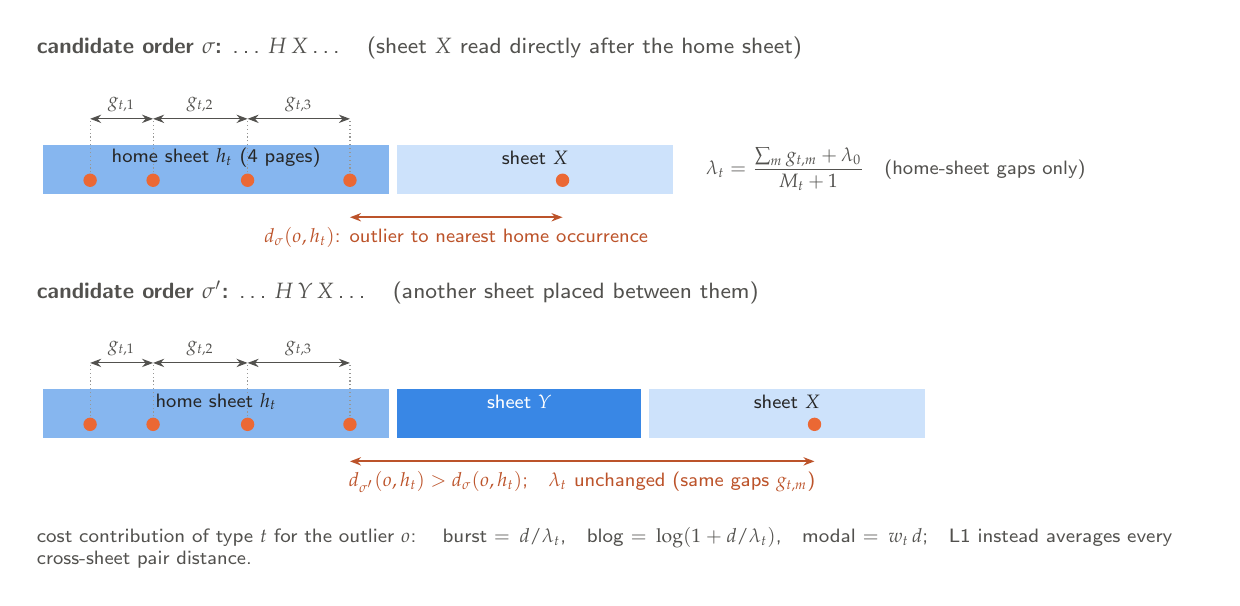
\begin{tikzpicture}[x=1cm,y=1cm,font=\sffamily\scriptsize,>={Stealth[length=4pt]}]
\begin{scope}[shift={(0,0)}]
\node[anchor=west,color=ink2,font=\sffamily\footnotesize] at (-0.2,1.85) {\textbf{candidate order $\sigma$:} \ldots\,$H$\,$X$\,\ldots\quad (sheet $X$ read directly after the home sheet)};
\fill[sheet2] (0,0) rectangle (4.4,0.62); \node[color=black!85] at (2.2,0.46) {home sheet $h_t$ (4 pages)};
\fill[sheet1] (4.5,0) rectangle (8.0,0.62); \node[color=black!85] at (6.25,0.46) {sheet $X$};
\foreach \x in {0.6,1.4,2.6,3.9}{\fill[accent] (\x,0.17) circle (0.085); \draw[ink2!60,densely dotted,thin] (\x,0.27) -- (\x,0.95);}
\fill[accent] (6.6,0.17) circle (0.085);
\foreach \a/\b/\l in {0.6/1.4/1,1.4/2.6/2,2.6/3.9/3}{\draw[<->,ink2] (\a,0.95) -- (\b,0.95) node[midway,above=-1pt]{$g_{t,\l}$};}
\draw[<->,accent!80!black,thick] (3.9,-0.3) -- (6.6,-0.3) node[midway,below]{$d_\sigma(o,h_t)$: outlier to nearest home occurrence};
\node[anchor=west,color=ink2] at (8.3,0.31) {$\lambda_t=\dfrac{\sum_m g_{t,m}+\lambda_0}{M_t+1}$ \; (home-sheet gaps only)};
\end{scope}
\begin{scope}[shift={(0,-3.1)}]
\node[anchor=west,color=ink2,font=\sffamily\footnotesize] at (-0.2,1.85) {\textbf{candidate order $\sigma'$:} \ldots\,$H$\,$Y$\,$X$\,\ldots\quad (another sheet placed between them)};
\fill[sheet2] (0,0) rectangle (4.4,0.62); \node[color=black!85] at (2.2,0.46) {home sheet $h_t$};
\fill[sheet3] (4.5,0) rectangle (7.6,0.62); \node[color=white] at (6.05,0.46) {sheet $Y$};
\fill[sheet1] (7.7,0) rectangle (11.2,0.62); \node[color=black!85] at (9.45,0.46) {sheet $X$};
\foreach \x in {0.6,1.4,2.6,3.9}{\fill[accent] (\x,0.17) circle (0.085); \draw[ink2!60,densely dotted,thin] (\x,0.27) -- (\x,0.95);}
\fill[accent] (9.8,0.17) circle (0.085);
\foreach \a/\b/\l in {0.6/1.4/1,1.4/2.6/2,2.6/3.9/3}{\draw[<->,ink2] (\a,0.95) -- (\b,0.95) node[midway,above=-1pt]{$g_{t,\l}$};}
\draw[<->,accent!80!black,thick] (3.9,-0.3) -- (9.8,-0.3) node[midway,below]{$d_{\sigma'}(o,h_t)>d_\sigma(o,h_t)$;\quad $\lambda_t$ unchanged (same gaps $g_{t,m}$)};
\end{scope}
\node[anchor=west,color=ink2,align=left,text width=14.8cm] at (-0.2,-4.5) {cost contribution of type $t$ for the outlier $o$: \; burst $=d/\lambda_t$,\quad blog $=\log(1+d/\lambda_t)$,\quad modal $=w_t\,d$;\quad L1 instead averages every cross-sheet pair distance.};
\end{tikzpicture}
\caption{The burst-scaled seriation cost. A rare type's home sheet holds most of its occurrences (orange); the gaps between them fix its burst scale $\lambda_t$ \cref{eq:lambda}, which is identical under every stacked order because a sheet's four pages are always contiguous. Each occurrence outside the home sheet contributes its distance to the nearest home occurrence, measured in units of $\lambda_t$ \cref{eq:burst}; the candidate order changes $d$, never $\lambda_t$.}
\label{fig:burstmetric}
\end{figure}

\subsection{Candidates, nulls and the best-of-$N$ heuristic}
\label{sec:nulls}

For each unit and cost the candidate vector $\mathbf{c}=(c(\sigma))_{\sigma}$ over all $S!$ stacked orders is standardised within itself, $z_\sigma=(c(\sigma)-\bar c)/s_c$, and the winner is $\sigma^\ast=\arg\min_\sigma c(\sigma)$ with $z^\ast=z_{\sigma^\ast}$. Three nulls are attached to it. \src{13--15}
\begin{itemize}
\item \textbf{Content shuffle.} Page contents are permuted among the quire's page slots (200 draws) and the best of all candidates is recomputed each time; $p_{\text{best}}$ is the empirical fraction \cref{eq:pemp} of shuffles whose winner is at least as extreme (in $z^\ast$) as the real winner. Page-level clumping is retained by construction.
\item \textbf{Geometry.} Page lengths stay in their slots and every occurrence of a rare type is re-placed uniformly over the quire's tokens (200 draws): does sheet \emph{size} alone favour the winning order? Valid for L1 and modal, which are means of distances; \emph{not} for burst and blog, whose $\lambda_t$ changes under uniform placement (their geometry $p$ is $\approx1$ everywhere and is discarded).
\item \textbf{Best-of-$N$.} The minimum of $N$ roughly normal candidate values is expected near $-\Phi^{-1}\!\bigl(1-\tfrac{1}{N+1}\bigr)$: about $-2.4$\,sd for $N=120$, $-3.0$ for 720, $-1.75$ for 24. A winner at that depth stands out from \emph{nothing}; the content-shuffle winners give the empirical version (\cref{sec:nullshape}).
\end{itemize}
Cross-unit consistency is the correlation of the candidate vectors of two units (e.g.\ words vs $n=7$) against the same correlation on shuffled contents, which keeps the overlap of $n$-grams with their words.

\paragraph{Power.} Known prose was written onto each quire's page slots, stacked in the current or a random sheet order, or nested (three texts $\times$ three windows). On quire M's slots the true stacked order ranks 1/120 in 4--6 of 18 cases and in the top 10 in 13 under L1 (median rank 6); the burst-scaled costs lower the median rank to 2--4 (burst 3/13, blog 6/13, modal 5/13 for rank-1/top-10). Written nested, the nested order ranks 1/121 in 8 of 9. Across the five quires, rank-1 counts (L1 / blog) are 6/6 (M), 1/2 (T; median rank 10/6 among 720), 6/5 (A), 4/4 (B), 5/3 (C), with top-10 in 13--15 of 18 on the four-to-five-sheet quires and 9--13 on T. So the metric recovers a prose writing order outright about a third of the time and usually to within the top tenth; with the manuscript's locality a tenth of prose (\cref{sec:baseline}), low power there is expected (\cref{fig:power}). A \textbf{nested-written control} asks which \emph{stacked} order prose written as bound prefers (L1, nine nested-written cases per quire): the bound order \order{1-2-\ldots-S} exactly in T 2/9, M 1/9, C 5/9, A 4/9, B 5/9 cases; an order within three pairwise inversions of it in T 6/9, M 8/9, C 9/9, A 9/9, B 9/9; an order with the outermost sheet adjacent to the innermost in T 1/9, M 3/9, C 4/9, A 4/9, B 0/9. So nested writing pulls the stacked seriation toward the bound order or a near variant, and produces the outermost-next-to-innermost feature at or below its chance rate (\cref{sec:seriation-results}). \src{13, 14, 15}

\begin{figure}[tbp]
\centering
\fig{fig_seriation_power}
\caption{Seriation power on known prose written onto each quire's page slots: rank of the true writing order among the candidate stacked orders (18 stacked-written cases per quire) under the four costs, and rank of the nested order among all candidates for nested-written prose. Nested-written control (L1, 9 cases per quire), best stacked order $=$ the bound order exactly: T 2/9, M 1/9, C 5/9, A 4/9, B 5/9; within three pairwise inversions of it: T 6/9, M 8/9, C 9/9, A 9/9, B 9/9; outermost sheet adjacent to innermost: T 1/9, M 3/9, C 4/9, A 4/9, B 0/9. \src{13--15}}
\label{fig:power}
\end{figure}

\subsection{Results}
\label{sec:seriation-results}

\paragraph{Stacked at all versus as bound.} On quire M, with all cross-page pairs, the nested binding ranks 100--121 of 121 on every unit and transcription (121/121 for $n=5,8$ on \IT\ and $n=7,8$ on \RF) and is no better than random page contents ($z$ $-0.6$ to $+0.9$), while the stacked candidates as a set beat shuffled contents at $z=+2.3$ to $+6.4$---the \cref{sec:leaf} result in seriation form: any reading that keeps a sheet's four pages together beats the binding, and the binding is as bad as chance. \src{13}

\paragraph{Which stacking.} \Cref{tab:quires} summarises the between-sheet seriation on the five quires; \cref{fig:quireT} details quire T and \cref{fig:quiresall} the $p$-grid. \src{14, 15}

\begin{table}[tbp]
\centering\footnotesize
\caption{Between-sheet seriation per quire (both transcriptions; $n$-gram units $n=5$--8 unless stated). Orders list sheets outer$\to$inner by number; ``bound-order rank'' is the rank of the current outer$\to$inner order \order{1-2-\ldots-S} among the $S!$ candidates. The reversal-equivalence used when these were first recorded is corrected in \cref{sec:direction}, which leaves the adjacency (which sheets neighbour which) unaffected. \src{14, 15}}
\label{tab:quires}
\setlength{\tabcolsep}{3pt}\renewcommand{\arraystretch}{1.1}
\begin{tabular}{@{}L{1.55cm}L{2.85cm}L{2.75cm}L{1.35cm}L{1.85cm}L{1.25cm}L{3.2cm}@{}}
\toprule
quire (sheets, orders) & $n$-gram best order & $p_{\text{best}}$, content shuffle & $z^\ast$ within candidates & $p$, geometry & bound-order rank & words (order; $p$)\\
\midrule
\textbf{T} (6, 720) & \textbf{\order{1-6-5-4-2-3}}\newline 31/32 cells$^{a}$ & L1 0.005--0.02\newline blog 0.005--0.02\newline modal 0.005--0.02 & $-3.1$ to $-4.05$ & L1 0.005\newline modal 0.005--0.02 & 150--626 & \order{1-6-5-4-3-2} (\IT)\newline \order{1-6-5-4-2-3} (\RF)\newline L1 0.005; modal 0.01--0.015; burst, blog 0.36--0.74\\
\addlinespace
M (5, 120) & \order{2-3-5-1-4}\newline \order{3-2-5-1-4}\newline \order{4-1-2-3-5}\newline one family$^{b}$ & L1 0.005--0.07\newline blog 0.01--0.12\newline modal 0.005--0.03 & $-2.3$ to $-3.2$ & L1 0.005--0.01\newline modal 0.005--0.03 & 30--114 & \order{2-3-5-1-4}\newline 0.03--0.4\\
\addlinespace
C (4, 24) & \textbf{\order{1-4-3-2}}\newline 30/32 cells & L1 0.005--0.15\newline blog 0.01--0.07\newline modal 0.005--0.27 & $-1.2$ to $-2.1$ & L1 0.005\newline modal 0.005--0.07 & 4--10 & \order{2-3-1-4}, \order{1-2-3-4}, \order{2-1-3-4}\newline 0.03--0.7\\
\addlinespace
A (4, 24) & split$^{c}$\newline \order{1-2-4-3}\newline \order{1-4-2-3}\newline \order{3-1-2-4} & L1 0.01--0.1\newline blog 0.035--0.26\newline modal 0.02--0.4 & $-1.4$ to $-2.2$ & L1 0.005\newline modal 0.01--0.9 & 10--20 & \order{2-4-1-3}\newline 0.1--0.5\\
\addlinespace
B (3 sheets + leaf f13, 24) & \order{1-2-3-4}, the bound order ($n=6$--8) & L1 0.18--0.65\newline blog 0.06--0.56\newline modal 0.11--0.75 & $-1.3$ to $-2.4$ & L1 0.005--0.17\newline modal 0.005--0.68 & 1--4 & \order{1-4-3-2} and others\newline 0.1--0.8\\
\bottomrule
\multicolumn{7}{@{}p{16cm}@{}}{\footnotesize $^{a}$\,The single exception is \IT\ $n=5$ under L1, burst and modal, which give \order{6-1-5-4-2-3} (sheets 1 and 6 swapped at the head of the chain). $^{b}$\,One family: sheets 2 and 3 (f76/f83, f77/f82) together, then 5 (f79/f80), then 1 (f75/f84), with 4 (f78/f81) at an end; \order{4-1-2-3-5} is the same family with sheet 1 moved next to sheet 4. $^{c}$\,\order{1-2-4-3} under L1 and burst at $n=5$--7; \order{1-4-2-3} at $n=7$--8; \order{3-1-2-4} under blog and modal at $n=5$--6.}
\end{tabular}
\end{table}

\begin{figure}[tbp]
\centering
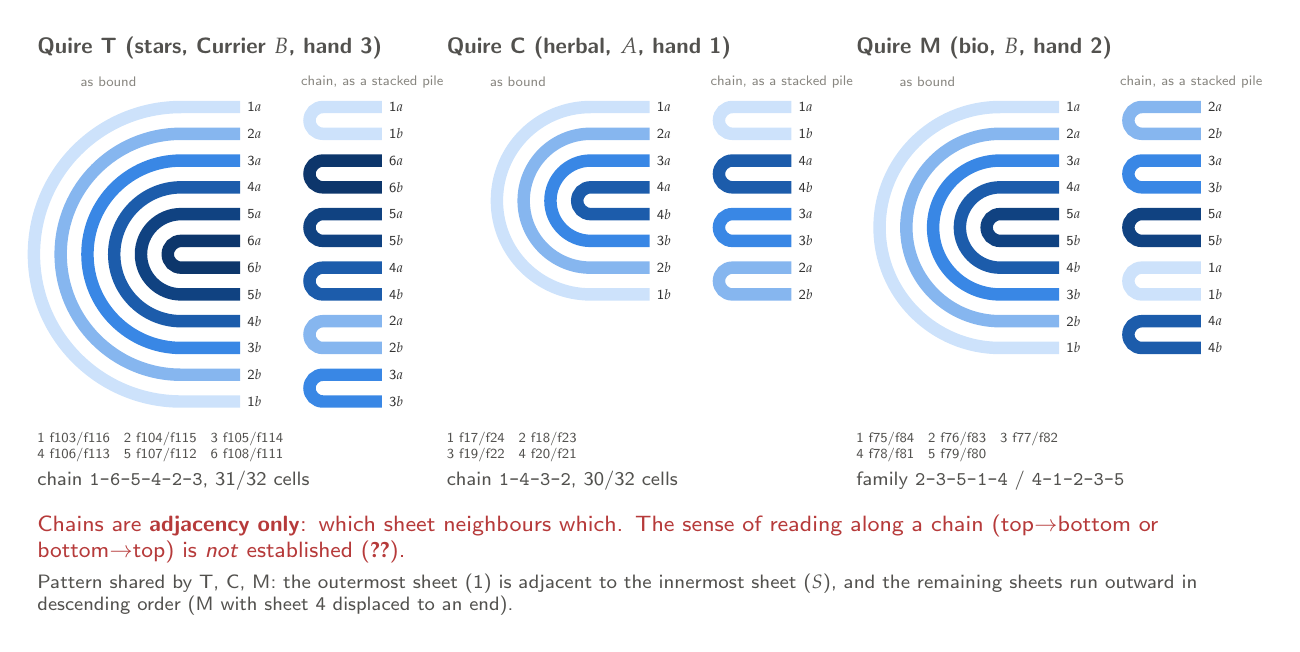
\begin{tikzpicture}[x=1cm,y=1cm,font=\sffamily\scriptsize,>={Stealth[length=4pt]}]
\renewcommand{\qpitch}{0.34}\renewcommand{\qarm}{0.75}\renewcommand{\qband}{4.5pt}
\newcommand{\quirebox}[6]{% x0, S, name, folios list (label), chain list, subtitle
\begin{scope}[shift={(#1,0)}]
\node[anchor=west,color=ink2,font=\sffamily\footnotesize\bfseries] at (0,0.75) {#3};
\node[anchor=west,color=muted,font=\sffamily\tiny] at (0.55,0.32) {as bound};
\node[anchor=west,color=muted,font=\sffamily\tiny] at (3.35,0.32) {chain, as a stacked pile};
\begin{scope}[shift={(1.95,0)}]\qnestedmini{#2}\end{scope}
\begin{scope}[shift={(3.75,0)}]\qstackedorder{#5}\end{scope}
\node[anchor=north west,color=ink2,align=left,font=\sffamily\tiny] at (0,-4.0) {#4\\[2pt] {\scriptsize #6}};
\end{scope}}
\quirebox{0}{6}{Quire T (stars, Currier $B$, hand 3)}{1 f103/f116 \; 2 f104/f115 \; 3 f105/f114\\4 f106/f113 \; 5 f107/f112 \; 6 f108/f111}{1,6,5,4,2,3}{chain \order{1-6-5-4-2-3}, 31/32 cells}
\quirebox{5.2}{4}{Quire C (herbal, $A$, hand 1)}{1 f17/f24 \; 2 f18/f23\\3 f19/f22 \; 4 f20/f21}{1,4,3,2}{chain \order{1-4-3-2}, 30/32 cells}
\quirebox{10.4}{5}{Quire M (bio, $B$, hand 2)}{1 f75/f84 \; 2 f76/f83 \; 3 f77/f82\\4 f78/f81 \; 5 f79/f80}{2,3,5,1,4}{family \order{2-3-5-1-4} / \order{4-1-2-3-5}}
\node[color=nestedc!80!black,anchor=north west,font=\sffamily\footnotesize,text width=15cm,align=left] at (0,-5.05) {Chains are \textbf{adjacency only}: which sheet neighbours which. The sense of reading along a chain (top$\to$bottom or bottom$\to$top) is \emph{not} established (\cref{sec:direction}).};
\node[color=ink2,anchor=north west,text width=15cm,align=left] at (0,-5.8) {Pattern shared by T, C, M: the outermost sheet (1) is adjacent to the innermost sheet ($S$), and the remaining sheets run outward in descending order (M with sheet 4 displaced to an end).};
\end{tikzpicture}
\caption{Sheet-adjacency chains selected by the seriation in quires T, C and M, drawn as in \cref{fig:codicology}. Left of each panel: the quire's sheets as bound (1 outermost); right: the same sheets each folded on their own and piled in the selected chain order, colour-coded by physical position. The outermost-next-to-innermost feature has chance rate $2/S$ under a random order ($1/3$ for T, $1/2$ for C), so it is informative for T and at chance for the four-sheet quires on its own; C's replication is the full chain \order{1-4-3-2}. \src{15}}
\label{fig:chains}
\end{figure}

\begin{description}
\item[Quire T is unambiguous by this test.] Every $n$-gram length, both transcriptions and all four costs choose \order{1-6-5-4-2-3} (words: \order{1-6-5-4-3-2}); it beats shuffled contents in $\le1$ of 200 draws on every cell, beats sheet geometry likewise, sits 3--4\,sd below the candidate mean where a random minimum of the candidate set would sit near 2.9, and the current outer$\to$inner order lies in the bottom half to bottom tenth of the 720. In folios: f103/f116, f108/f111, f107/f112, f106/f113, f104/f115, f105/f114. \src{15}
\item[Quire C replicates the shape] with a smaller quire in a different language, hand and section: \order{1-4-3-2} on 30 of 32 cells, $p$ 0.005--0.05 on most, geometry excluded. \src{15}
\item[Quire M is consistent.] The plain mean (L1) found the best of 120 orders exactly as deep as the best of random values and a different optimum per unit \src{13}; the burst-scaled costs make the $n$-gram units agree on one family---sheets 2 and 3 (f76/f83, f77/f82) together, then 5 (f79/f80), then 1 (f75/f84), then 4 (f78/f81) at the end, or \order{4-1-2-3-5} with 1 moved next to 4---with the best-of-120 beating shuffled contents at $p$ 0.005--0.05 in 14 of 16 $n$-gram $\times$ cost $\times$ transcription cells (modal 8/8 at $\le0.035$). The words stay weak ($p$ 0.1--0.4). The between-sheet affinity matrix (shared rare pairs, observed/expected) reads the same way: sheets 1 and 5 share most (1.35--1.42 words, 1.04--1.08 at $n=7$), 2--3, 3--5 and 2--5 share 1.1--1.2, and sheet 4 shares least with everything (0.63--0.87, except 1.0 with sheet 1). \src{13, 14}
\item[Quire A] shows sharing above shuffled contents (L1 $p$ 0.01--0.05, geometry excluded) but no single order; the current order is disfavoured. \textbf{Quire B} (three sheets and a leaf, 1\,000 tokens) prefers its current order but not above shuffled contents: no information. \src{15}
\end{description}

\begin{figure}[tbp]
\centering
\fig{fig_quire_T}
\caption{Quire T. (a)~Histogram of the within-candidate $z$ of the 720 stacked orders on the real contents and on shuffled contents, with the winner \order{1-6-5-4-2-3} and its sheet-reversal marked. (b)~The winner's $z^\ast$ per unit and transcription against the distribution of shuffled-content winners, with the empirical $p$. (c)~Between-sheet affinity matrices (shared rare pairs, observed/expected; words and 7-grams, \IT) with the chain's adjacencies framed. The recorded JSON holds summaries only, so the candidate vectors and affinities were re-derived with the recorded code (\texttt{figures/derive\_quire\_T.py}, output \texttt{data/derived\_quire\_T\_costs.json}, fresh null seed); the recorded $z^\ast=-3.96$ for $n=7$ under L1 is reproduced exactly. \src{15, 17}}
\label{fig:quireT}
\end{figure}

\begin{figure}[tbp]
\centering
\IfFileExists{figures/fig_quires_all.pdf}{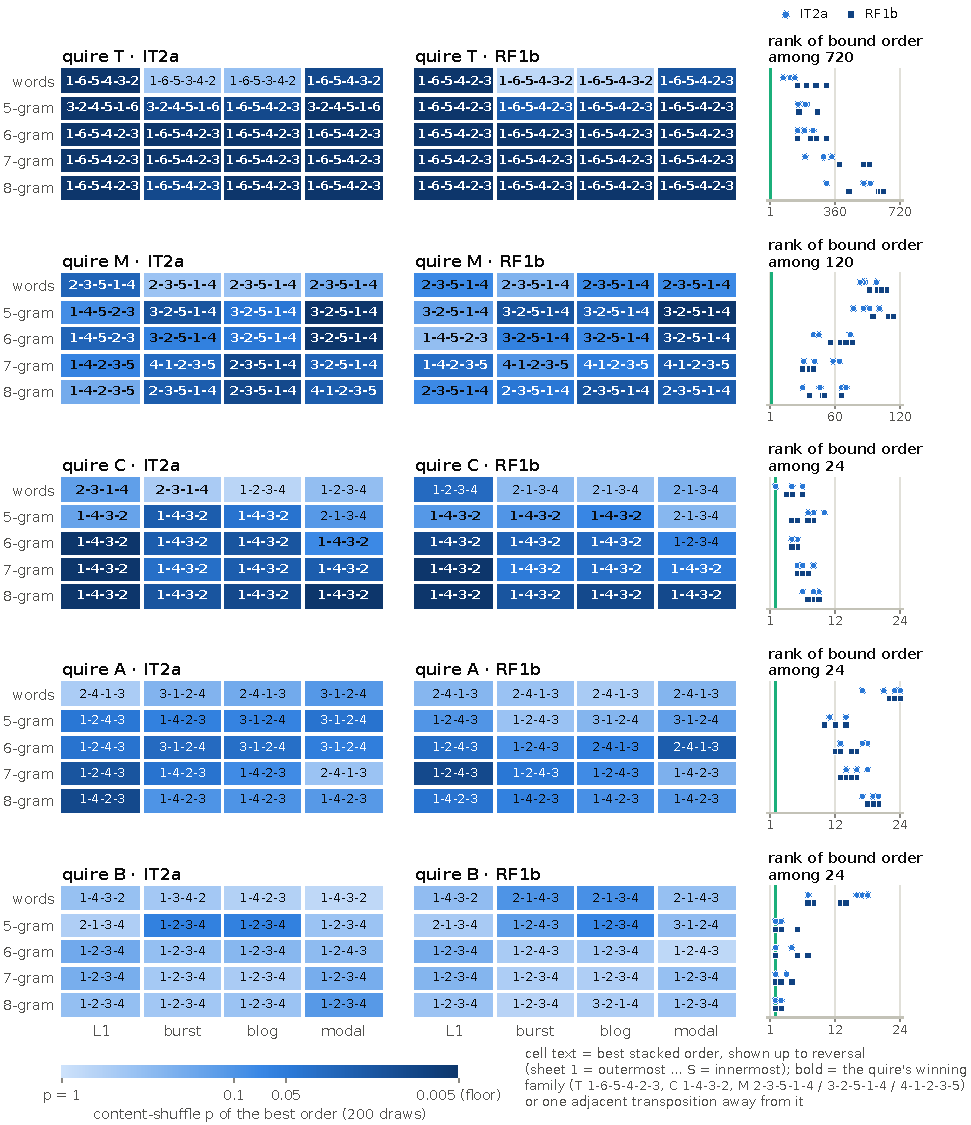
\includegraphics[width=\textwidth,height=0.82\textheight,keepaspectratio]{fig_quires_all}}{\fbox{\parbox[c][3cm][c]{0.9\linewidth}{\centering\sffamily\color{muted}figure not yet generated}}}
\caption{All five quires: content-shuffle $p_{\text{best}}$ of the winning order per unit and cost (log colour scale; floor $1/201$), both transcriptions, with the winning order and the rank of the current outer$\to$inner order. \src{14, 15}}
\label{fig:quiresall}
\end{figure}

\paragraph{The pattern across T, C and M.} The outermost sheet sits next to the innermost sheet, and the remaining sheets then run outward in descending order: T \order{1-6-5-4-2-3} ($n$-grams; words \order{1-6-5-4-3-2}), C \order{1-4-3-2}, M \order{4-1-5-3-2} (words, $n=8$; the sheet-reversal of the \order{2-3-5-1-4} of \cref{tab:quires}, written this way round to show the pattern) with sheet 4 displaced to the front (\cref{fig:chains}). Two chance rates qualify the pattern. Under a uniformly random sheet order the outermost and innermost sheets are adjacent with probability $2/S$: $1/3$ for T ($S=6$) and $1/2$ for the four-sheet quires C and A. The feature is therefore informative for T---where nested-written prose shows it in 1 of 9 cases and the bound order is at chance---and, taken on its own, at chance for C and A; what C replicates is a specific full chain (\order{1-4-3-2} on 30 of 32 cells), not this feature. Nested-written prose does not produce the chains (its best stacked order is the bound order or a near variant, \cref{sec:nulls}), and neither sheet geometry nor page-level clustering does (the content shuffle keeps each page's own bursts). What could: composition sheet by sheet in that order; or a chain of sheet-level subject affinities that happens to run outermost $\to$ innermost $\to$ outward. The test cannot tell the two apart. \src{15}


%=====================================================================
\section{Other ways of gathering the sheets}
\label{sec:nesting}

\Cref{sec:leaf,sec:seriation} compared the stacked orders with one nested arrangement, the binding. Two alternatives were left open: the same sheets nested in a different order, and a quire made of two or three smaller nested gatherings laid one after another. Both would keep some conjugate leaves apart and might describe the rare-material locality as well as the stacked optimum does. Here every such pattern is a candidate. \src{19}

\paragraph{Pattern space.} An order $\sigma$ of the $S$ sheets is cut into consecutive blocks, and each block is nested: its sheets' $a$-leaves outer$\to$inner, then their $b$-leaves inner$\to$outer. A block of one sheet is that sheet read stacked, so the fully stacked orders ($S$ blocks) and the fully nested ones (one block, the binding among them) are the two extremes of one space of
\begin{equation}
N_S = S!\;2^{\,S-1}
\label{eq:patterns}
\end{equation}
page sequences: 192 for a four-sheet quire, 1\,920 for M, 23\,040 for T (quire B has 144 distinct sequences, because its fourth ``sheet'' is the single leaf f13 and a block that starts with it reads the same as stacking it before the block). Labels write blocks between bars with sheets outer$\to$inner inside a block: \order{1|4|3|2} is stacked, \order{1432} nested, \order{14|32} two nested pairs.

\paragraph{Cost, and a bias to declare.} A nested block separates a sheet's two leaves, so the within-sheet distances are no longer constant across candidates and the pair set of \cref{sec:costs} cannot be reused. The cost for this question is the mean distance over \emph{all} cross-page occurrence pairs of rare types,
\begin{equation}
c_{\mathrm{L1}}(\pi)=\frac{1}{|P|}\sum_{(i,j)\in P} d_\pi(i,j),
\label{eq:l1all}
\end{equation}
the ``stacked at all versus as bound'' setting of \cref{sec:seriation} extended to the whole space. The burst-scaled costs were also run, with a home-cluster term added (every home occurrence to its nearest other home occurrence) that charges any pattern splitting a home sheet. That family is \textbf{structurally biased toward stacked patterns} here: on shuffled contents its winner is fully stacked in 76--100\,\% of draws on the $n$-grams, because the home sheet is by definition the sheet holding most of a type's occurrences and keeping its four pages contiguous minimises the home term whatever the content; and nested-written prose is never ranked first by it in 27 controls. The L1 cost has no such bias---its shuffled-content winners fall on the block classes in proportion to class size (fully nested winners 6--7\,\% of null draws in M against $120/1\,920=6.3\,\%$ of the space; 12--17\,\% in the four-sheet quires against $24/192=12.5\,\%$) and it recovers nested writing when prose is written nested (below). So L1 is the cost for the class question and the burst family is used only as a check of the ranking within the stacked class, where it reproduces \cref{sec:seriation-results}. The null is the content shuffle of \cref{sec:nulls} (200 draws; 100 on T) with the best of all patterns recomputed each time; three statistics are compared with their own null: the winner's $p_{\text{best}}$, the \emph{gain} of the full space over the best stacked order (in candidate sd), and the \emph{margin} by which the best fully nested order trails the best stacked order, with $P(\text{chance})$ the fraction of shuffles producing a margin at least as large.

\paragraph{Power.} Known prose written onto each quire's page slots (three texts $\times$ three windows, words, L1). Written as bound, the binding ranks 1 of 192 in 2/9 (C), 1/9 (A) and 3/9 (B) cases, 0/9 of 1\,920 (M) and 1/9 of 23\,040 (T); written nested in a random sheet order, that order ranks 1 in 4/9, 0/9, 2/9, 0/9, 1/9; a random two-block pattern 1/9, 0/9, 1/9, 1/9, 1/9; a random stacked order 1/9, 1/9, 0/9, 1/9, 1/9. Median ranks are 9--27 in every mode (T's stacked-random 134 of 23\,040). The cost identifies the writing \emph{pattern} about as well as it identified the writing \emph{order} in \cref{sec:nulls}, with no preference among the four kinds: prose written nested is won by a nested pattern, prose written stacked by a stacked one. \src{19}

\begin{table}[tbp]
\centering\footnotesize
\setlength{\tabcolsep}{3pt}
\caption{Every nesting pattern of a quire's sheets (L1 cost, \cref{eq:l1all}; ranges over the five units words, $n=5$--8; both transcriptions). ``Blocks in winner'' is the number of nested blocks in the overall winner per unit ($S$ = fully stacked). ``Gain'' is how far the overall winner lies below the best stacked order, in candidate sd, with the fraction of shuffled contents whose winner gains at least as much (a gain at $p\ge0.7$ is the ordinary effect of searching 8--32 times more candidates). ``Margin'' is how far the best fully nested order trails the best stacked one, with $P(\text{chance})$ from the same shuffles. \src{19}}
\label{tab:nesting}
\resizebox{\textwidth}{!}{%
\begin{tabular}{@{}llcccccc@{}}
\toprule
quire ($S$, $N_S$) & transcr. & \makecell{blocks in winner\\words/n5/n6/n7/n8} & \makecell{gain over best\\stacked, sd ($p$)} & \makecell{rank of\\best stacked} & \makecell{rank of best\\fully nested} & \makecell{rank of\\binding} & \makecell{margin nested $-$\\stacked, sd ($P$)}\\
\midrule
A (4, 192) & \IT & 3/4/3/3/3 & 0.00--0.13 (0.80--1.00) & 1--3 & 14--41 & 31--177 & +0.8 to +1.2 (0.12--0.36)\\
 & \RF & 4/3/4/3/3 & 0.00--0.08 (0.90--1.00) & 1--2 & 25--50 & 36--183 & +1.2 to +1.4 (0.09--0.15)\\
B (4, 144) & \IT & 2/4/4/4/4 & 0.00--0.79 (0.33--1.00) & 1--8 & 3--90 & 3--125 & $-$0.3 to +3.0 (0.00--0.74)\\
 & \RF & 2/4/4/4/4 & 0.00--0.69 (0.40--1.00) & 1--12 & 5--88 & 5--124 & $-$0.3 to +2.9 (0.00--0.74)\\
C (4, 192) & \IT & 3/3/4/4/4 & 0.00--0.32 (0.71--1.00) & 1--3 & 17--100 & 17--123 & +1.0 to +1.9 (0.05--0.16)\\
 & \RF & 3/3/4/4/4 & 0.00--0.02 (0.92--1.00) & 1--2 & 19--106 & 19--145 & +1.0 to +2.2 (0.03--0.23)\\
M (5, 1\,920) & \IT & 4/4/4/4/5 & 0.00--0.38 (0.71--1.00) & 1--13 & 650--818 & 1\,404--1\,862 & +2.3 to +2.6 (0.00--0.07)\\
 & \RF & 5/4/3/4/5 & 0.00--0.41 (0.72--1.00) & 1--24 & 177--881 & 1\,569--1\,887 & +1.5 to +2.7 (0.03--0.10)\\
T (6, 23\,040) & \IT & 4/6/6/6/6 & 0.00--0.18 (0.90--1.00) & 1--5 & 1\,750--10\,535 & 13\,942--22\,405 & +1.9 to +4.7 (0.01--0.05)\\
 & \RF & 5/6/6/6/6 & 0.00--0.16 (0.95--1.00) & 1--2 & 3\,588--8\,434 & 16\,868--21\,492 & +3.0 to +4.6 (0.01--0.02)\\
\bottomrule
\end{tabular}}
\end{table}

\begin{figure}[tbp]
\centering
\fig{fig_nesting}
\caption{Every nesting pattern of a quire's sheets, L1 cost. (a)~Best cost per number of nested blocks (1 = fully nested, $S$ = fully stacked), standardised within each quire's candidate set, $n=7$ glyph $n$-grams; the binding's own value is the red tick. The cost falls monotonically toward the stacked end in every quire and on both transcriptions. (b)~Margin by which the best fully nested order trails the best stacked order, per quire and unit, against the 5--95\,\% band of the same margin on shuffled contents. (c)~Rank of the best fully nested order (filled) and of the binding (hollow red) among all patterns, with the best stacked order's rank (aqua tick). \src{19}}
\label{fig:nesting}
\end{figure}

\paragraph{Results.} \Cref{tab:nesting,fig:nesting}. \textbf{Quire T (23\,040 patterns) is the decisive case.} A fully stacked order wins the whole space on every $n$-gram unit and both transcriptions---\order{3|2|4|5|6|1}, the un-folded optimum of \cref{sec:direction}, on seven of the eight cells and \order{3|2|4|5|1|6} on the eighth (\IT, $n=5$)---at $p_{\text{best}}=0.01$ against the shuffled winner. On the $n$-grams the best fully nested order ranks 5\,007--10\,535 (\IT) and 6\,146--8\,434 (\RF), the binding 19\,180--22\,405 and 17\,902--21\,492, and the nested class trails the stacked optimum by 3.4--4.7\,sd where shuffled contents give +0.7 to +0.9 ($P(\text{chance})=0.01$ on all eight $n$-gram cells, 0.02--0.05 on words). Nothing in the full space improves on the best stacked order: the shuffled winner typically beats its own best stacked order by 0.9--1.2\,sd through the wider search, the manuscript's by 0.00 on the $n$-grams and 0.16--0.18 on words ($p$ 0.90--0.95). In every quire and both transcriptions the overall winner is fully stacked or a pattern with one nested pair among otherwise stacked sheets (A's \order{1|42|3}, M's \order{14|5|2|3}, C's \order{2|13|4} on words), and where it is not fully stacked it beats the best stacked order by 0.02--0.4\,sd, exactly what the enlarged search gains on shuffled contents ($p$ 0.7--1.0 in every $n$-gram cell; the only values below 0.5 are quire B's words, a null cell where nothing is significant, $p_{\text{best}}$ 0.4--0.7). No fully nested order comes close: the best of them ranks 14--106 of 192 in the herbal quires (B's words excepted), 177--881 of 1\,920 in M and 5\,007--10\,535 of 23\,040 in T, and the binding ranks lower still. The nested class trails the stacked optimum by 1--3\,sd in the smaller quires, which shuffled contents reproduce in 3--15\,\% of draws on most $n$-gram cells (M \IT{} 0.005--0.07, C 0.03--0.23, A 0.09--0.36). Two-block patterns---the natural ``two smaller gatherings'' reading---never win on an $n$-gram unit anywhere. \src{19}

\paragraph{Reading.} The comparison of \cref{sec:leaf,sec:seriation} was not a straw man. What the rare material rewards is the property every stacked order shares, a sheet's four pages together, and no other way of gathering the same sheets---reordered nesting, two or three nested sub-gatherings, or a mixed pattern---recovers it. Within the stacked class the T chain of \cref{sec:seriation-results} stands as recorded (adjacency only; direction in \cref{sec:direction}). Two limits. The burst-family costs cannot be used for the class question at all (the bias above), so this section rests on L1 alone. And the space does not contain inverted folding combined with nesting, which nobody has proposed; a nested pattern whose leaves coincide with the stacked adjacency is already in it, since a sheet nested inside a one-sheet block is that sheet stacked. \src{19}

\section{Direction}
\label{sec:direction}

\subsection{An order and its sheet-reversal are not equivalent}

When the seriation results were first recorded, an order and its sheet-reversal were treated as equivalent and each best order reported as the smaller label of the pair. That is wrong: reversing the sheet order does not reverse the page sequence, because every sheet is still read $a^r,a^v,b^r,b^v$. For a type with an occurrence at within-sheet position $x$ in sheet $A$ (length $L_A$) and one at $y$ in sheet $B$ (length $L_B$),
\begin{equation}
d_{AB}=(L_A-x)+y,\qquad d_{BA}=(L_B-y)+x,\qquad d_{AB}-d_{BA}=(L_A-L_B)-2(x-y),
\label{eq:direction}
\end{equation}
so shared types falling \emph{late} in one sheet and \emph{early} in the next favour that reading sense. Summed over pairs, this asymmetry is the direction signal; it is a small part of the between-sheet distance (the within-sheet position, against whole-sheet offsets of $\approx$700 tokens), and the adjacency results of \cref{sec:seriation} are unaffected (reversal pairs differ by $\le2$\,sd and were always ranked together). \src{16}

\subsection{The gap to the reversal and its null}

For each unit and cost the un-folded winner $\sigma^\ast$, its reversal $\bar\sigma^\ast$, the reversal's rank, and the gap
\begin{equation}
\Delta=\frac{c(\bar\sigma^\ast)-c(\sigma^\ast)}{s_c}\ \ (\text{in candidate sd})
\label{eq:delta}
\end{equation}
are computed. Because \emph{any} winner beats its reversal by construction, the null for $\Delta$ is taken from each content shuffle's own winner and \emph{its} reversal (200 draws)---the same selection, so the selection bias is inside the null---and $p$ is the fraction of shuffles with a gap at least as large. \src{16}

\begin{table}[t]
\centering\small
\caption{Direction test: un-folded winner, rank of its reversal, gap $\Delta$ \cref{eq:delta} and its selection-matched null. \src{16}}
\label{tab:direction}
\footnotesize\setlength{\tabcolsep}{4pt}\renewcommand{\arraystretch}{1.08}
\begin{tabular}{@{}lL{5.6cm}cccc@{}}
\toprule
quire & un-folded best ($n=5$--8, both transcriptions; L1 $\cdot$ blog $\cdot$ modal) & reversal's rank & $\Delta$ (sd) & null $\Delta$ (sd) & $p$\\
\midrule
T & \textbf{\order{3-2-4-5-6-1}} in 22 of 24 L1$\cdot$blog$\cdot$modal cells (29 of 32 including burst); exceptions \IT\ $n=5$ L1/burst/modal \order{3-2-4-5-1-6}; words \order{2-3-4-5-6-1} / \order{3-2-4-5-6-1} & 5--27 / 720 & 0.6--1.7 & 0.8--1.4 $\pm$ 0.5--0.7 & 0.20--0.80\\
\addlinespace
M & inconsistent: \order{2-3-5-1-4}, \order{4-1-5-2-3}, \order{1-4-5-2-3}, \order{1-4-2-3-5}, \order{4-1-2-3-5} & 2--35 / 120 & 0.1--2.1 & 0.8--1.5 & 0.07--0.98\\
\addlinespace
C & \order{1-4-3-2} ($n=6$--8), \order{2-3-4-1} ($n=5$) & 2--6 / 24 & 0.05--1.1 & 1.1--1.6 & 0.66--1.00\\
A & \order{3-1-2-4} / \order{1-2-4-3} / \order{1-4-2-3}, split & 2--8 / 24 & 0.0--0.9 & 1.0--1.5 & 0.55--1.00\\
B & \order{1-2-3-4} and \order{4-3-2-1} both appear & 2--9 / 24 & 0.0--1.5 & 1.0--1.3 & 0.38--1.00\\
\bottomrule
\end{tabular}
\end{table}

No quire's direction is established (\cref{tab:direction}, \cref{fig:direction}a): every gap between the best order and its reversal is the size that selecting the best of the candidate set produces on shuffled contents ($p\ge0.07$, mostly $\ge0.3$). Quire T's direction is at least \emph{consistent}---\order{3-2-4-5-6-1} in 22 of 24 L1$\cdot$blog$\cdot$modal cells (29 of 32 with burst; the exceptions are the \IT\ $n=5$ cells, \order{3-2-4-5-1-6}), i.e.\ f105/f114, f104/f115, f106/f113, f107/f112, f108/f111 and the outermost f103/f116 \emph{last}---but the cells are correlated and the gap is ordinary; and ``the outermost sheet holds the end'' is also where a text written as bound ends (f116). \src{16}

\subsection{Is there a time arrow inside a burst?}
\label{sec:frontloading}

The only route to direction that does not depend on the sliver of within-sheet position in \cref{eq:direction} would be burst \emph{shape}: if a rare type is introduced, reused quickly and tails off, a burst straddling a sheet boundary tells from its shape which sheet came first. For every type with 3--10 occurrences inside one segment, two statistics were taken: the fraction of types whose first inter-occurrence gap is shorter than the last (front-loaded $\Rightarrow>0.5$; sign test) and the skew $(\bar x-\tfrac{x_1+x_k}{2})/(x_k-x_1)$ (front-loaded $\Rightarrow<0$; $t$-test). Segments were 1\,500-token windows of six known texts (words and character 5--8-grams), the manuscript's 50 sheets of $\ge3$ pages read $a^r,a^v,b^r,b^v$ (direction known, no order search), by Currier language, and its pages; the control puts the four pages of every four-page sheet in random order (200 draws), keeping every page-level effect and destroying only the reading order. \src{18}

\textbf{Prose has no usable arrow.} Pooled over six texts, the first$<$last fraction is 0.503 for words ($n=19\,551$) and 0.502--0.508 for $n$-grams, skew $-0.0004$ to $-0.0011$; by text the fraction ranges 0.48--0.53 with both signs. The only trace is in long $n$-grams with $\ge5$ occurrences (0.52--0.55), a few per cent. A burst is, to within a per cent, symmetric in time, so the premise fails and the shape of a straddling burst cannot give direction anywhere. The manuscript is symmetric too (all sheets pooled 0.49--0.51; pages 0.48--0.51; Currier $B$ sheets 0.49--0.50, permutation $p$ 0.17--0.61). The one asymmetry---Currier $A$ herbal sheets, $n$-grams only, back-loaded at 0.44--0.47, driven by $k=3$ types, $p$ 0.005--0.1 against the within-sheet page permutation on six correlated cells, both transcriptions---is not the mirror of any prose property (prose $k=3$ is 0.50 exactly) and so is not evidence that $A$ sheets are read backwards; its shape is what a \emph{leaf-level} difference would produce (the two pages of leaf $b$ sharing rare $n$-grams more than the two pages of leaf $a$), a layout or production question given that herbal $a^r$ pages carry the large drawings. Page length in $A$ sheets falls $104\to95\to87\to82$ tokens by position, but the permutation null carries lengths with the pages and still gives 0.50. \src{18}

\begin{figure}[tbp]
\centering
\fig{fig_direction}
\caption{Direction. (a)~Gap $\Delta$ between the winning order and its sheet-reversal (in candidate sd) against the selection-matched null from shuffled contents, per quire and unit. (b)~Burst front-loading: fraction of rare types whose first gap is shorter than the last, for known texts and for the manuscript's sheets and pages; 0.5 is symmetry. The two grey bands are the range of the pooled prose value over the five units and the range of the six individual prose texts. \src{16--18}}
\label{fig:direction}
\end{figure}

%=====================================================================
\section{Shape of the nulls}
\label{sec:nullshape}

The ``$\pm$sd'' summaries and the best-of-$N$ heuristic were checked against the actual null distributions on quires T, M and C (\IT, 200 content shuffles, L1 and modal). \src{17}
\begin{itemize}
\item \textbf{Candidate cost vector.} On shuffled contents it is near-normal but mildly flat: skew $\approx0$, excess kurtosis $-0.3$ to $-0.8$; Shapiro--Wilk rejects at 5\,\% in 6--34\,\% of shuffles for M (120 orders) and C (24), and in 80--92\,\% for T (720 orders, where the test has power against the flatness). On the \emph{real} contents T's vector is clearly non-normal (skew $-0.4$ to $-1.0$, kurtosis up to $+0.8$ at $n=6$--7): a left tail of low-cost orders---the winning family itself---which is the signal, not a null defect. M's real vectors are mildly left-skewed ($-0.1$ to $-0.6$), C's mildly right-skewed.
\item \textbf{Winner's within-candidate $z$.} Median $z^\ast$ of the shuffled winner: M $-2.26$ to $-2.42$ (Gaussian heuristic $-2.40$), C $-1.80$ to $-1.91$ ($-1.75$), T $-2.65$ to $-2.98$ ($-2.99$). The heuristic was adequate. Empirical $p$ of the real winner's $z^\ast$ against the shuffled winners': T $n=6$--8 $p$ 0.005--0.015 (both costs), $n=5$ 0.045 / 0.16, words 0.13--0.15; M modal $n=5$ 0.005, $n=6$ 0.07, the rest 0.16--0.51; C 0.50--0.97---matching the $p_{\text{best}}$ values of \cref{tab:quires}, which were already empirical.
\item \textbf{Direction gap $\Delta$.} Bounded at zero and right-skewed (skew $+0.2$ to $+1.3$; median 0.7--1.4\,sd, upper quartile 1.0--2.0, maxima 2.2--4.0), so ``mean $\pm$ sd'' was a poor summary; the empirical $p$ of \cref{tab:direction} stands. The real $\Delta$ falls inside the null interquartile range on every T cell ($p$ 0.20--0.83) and on C ($p$ 0.48--0.99); M's only low cell is $n=7$ L1 at $p$ 0.085.
\end{itemize}
Nothing in \cref{sec:seriation,sec:direction} rests on normality: the candidate distribution's departure from normal in T is the finding, and the gap distribution's departure is why only the empirical $p$ was ever quoted.

%=====================================================================
\section{Discussion}
\label{sec:discussion}

\begin{establishes}
\begin{enumerate}
\item The manuscript's rare vocabulary has about one tenth of the passage-scale locality of prose and clusters like rhymed verse at every frequency class $k=2$--5 and in both Currier languages (\cref{sec:baseline}).
\item Despite that, the sheet is a unit that shares rare material: conjugate leaves share more, nested neighbours share less, on words and on glyph $n$-grams, on both transcriptions, with quire, language and hand held fixed (\cref{sec:leaf}). Six real texts reproduce the sign and size only when written sheet by sheet (36/36 vs 36/36). No other way of gathering the same sheets does as well: over every reordered, sub-gathered and mixed nesting of a quire's sheets (up to 23\,040 patterns) nothing beats the best stacked order beyond what the wider search gains on shuffled contents, the best fully nested order ranks 5\,007--10\,535 of 23\,040 in T, and the binding lower still (\cref{sec:nesting}).
\item The effect is small in mass---rare types are not contained by sheet, solver windows are unchanged, no sheet order lifts the locality above the noise ceiling (\cref{sec:isnot})---and lives in the $\sim$20\,\% of pairs that fall within a quire.
\item Within a quire the burst-scaled seriation selects a sheet chain in T (\order{1-6-5-4-2-3}, 31/32 cells, $p\le0.02$ against shuffled contents and geometry), replicates the shape in C (\order{1-4-3-2}) and is consistent in M; in each the outermost sheet neighbours the innermost---informative for T (chance rate $2/S=1/3$; nested-written prose 1/9), at chance ($1/2$) for the four-sheet quires on its own, so C's contribution is the full chain rather than this feature (\cref{sec:seriation}).
\end{enumerate}
\end{establishes}

\begin{notestablished}
\begin{enumerate}
\item \textbf{Composition unit versus work unit.} Every statistic here responds equally to ``the text flows $a^r\to a^v\to b^r\to b^v$ across the sheet'' and to ``one scribe, one session, one topic per sheet, with the intended reading order still nested''. The hands running by sheet (97\,\% of conjugate pairs same hand) is itself evidence that the sheet was a working unit. A rare-material statistic cannot separate the two; that is what Davis's stacked proposal and a sheet-level production account share.
\item \textbf{Direction.} The sense of reading along any chain is not established (\cref{sec:direction}): the gap to the reversal is what selection produces on noise, and prose bursts are symmetric to within a per cent, so there is no arrow to calibrate on.
\item \textbf{Which sheets or quires are misplaced.} The per-quire word-level picture is uneven (signal in A, T, H, M; none in herbal B--G); quires D--G (mixed language/hand), O, Q and S were not seriated; the codicological literature's specific reorderings were not tested as fixed candidates; T's chain has not been checked against the codicology (f103/f116 is the sheet with the missing f116v text).
\item \textbf{A stacking that recovers prose-like locality.} None exists: the separation from prose is within the sheet (\cref{sec:optimize}).
\end{enumerate}
\end{notestablished}

\paragraph{Sequential testing and correlated cells.} The evidential order matters. The doubleton test was null; the pooled-word statistic was chosen after seeing it ($p\approx0.01$, not pre-registered); the $n$-gram test was then run as the pre-stated check and is the number to quote ($z=+3$ to $+5$, 0/5\,000 even-spread draws at $n\ge7$, hand-controlled). Within every table the cells are correlated: $n$-grams of neighbouring $n$ overlap, the two transcriptions are one text, the three burst-scaled costs share their outliers, the nesting-pattern cells of \cref{sec:nesting} share their candidates with the stacked seriation, and the herbal quires' candidate sets are tiny (24 orders), so their $p$-values are coarse. Quire T's seriation is the result to quote; C is a replication in a different language, hand and section; M is consistent; A and B are uninformative.

\paragraph{What would settle it.} (i)~An independent quire-internal signal reaching the same optimum---the words alone at $p<0.05$ in T or M, or a whole-vocabulary leaf similarity with language and section controlled. (ii)~The specific reorderings proposed in the codicological literature run as fixed candidates against the within-quire null, instead of a search over all $S!$. (iii)~The remaining multi-sheet quires. (iv)~A production-side test of the composition-vs-work distinction that does not use text position at all (ink, ruling, drawing sequence). (v)~For the Currier-$A$ $n$-gram back-loading, the one follow-up worth running before any interpretation: within-leaf sharing, leaf $a$ versus leaf $b$, on the herbal quires. (vi)~The latent-semantic-analysis test Davis reported (\cref{sec:question}), should it be published: a page-level topic similarity is the natural complement to a rare-type position statistic, and agreement or disagreement on the sign of the conjugate-versus-nested contrast would be informative either way. None of this needs the GPU; every run here is seconds to minutes on CPU.

%=====================================================================
\appendix
\section{Reproduction}
\label{app:repro}

All artifacts referenced below are copied into the report folder's \texttt{data/} directory (from the analysis root's \texttt{analysis/doubleton\_gaps/}); the analysis scripts live in the repository's \texttt{scripts/} directory and are run as
\begin{center}\texttt{uv run python scripts/<name>.py}\end{center}
Figures are rebuilt with \texttt{make figures} (one script per figure under \texttt{figures/}, shared style in \texttt{style.py}); the document with \texttt{make}.

\begin{table}[H]
\centering\small
\caption{Analysis scripts, their artifacts and the sections they support.}
\label{tab:scripts}
\footnotesize\setlength{\tabcolsep}{4pt}
\begin{tabular}{@{}L{5.5cm}L{6.8cm}L{3.4cm}@{}}
\toprule
script & artifacts (\texttt{data/}) & report section (record \S)\\
\midrule
\texttt{doubleton\_gaps.py} & \texttt{summary.json}; \texttt{vms\_*\_doubletons.csv};\newline\texttt{page\_affinity\_*.csv} & \cref{sec:baseline} (2, 3, 4)\\
\texttt{doubleton\_leaf\_affinity.py} & \texttt{leaf\_affinity.json};\newline\texttt{leaf\_affinity\_controls.json} & \cref{sec:leaf} (4)\\
\texttt{rare\_type\_clustering.py} & \texttt{rare\_types.json};\newline\texttt{rare\_types\_controls.json}; logs & \cref{sec:baseline,sec:leaf} (6)\\
\texttt{glyph\_ngram\_leaf\_test.py} & \texttt{glyph\_ngrams.json}; \texttt{hand\_control.json}; logs & \cref{sec:leaf,sec:hand} (7)\\
--- & \texttt{window\_tokens\_per\_type.log}; \texttt{containment.log}; \texttt{corpus\_sweep.json} & \cref{sec:isnot,sec:baseline} (8, 9, 11)\\
\texttt{order\_optimize.py} & \texttt{order\_optimize\_none.json};\newline\texttt{order\_optimize\_inverted.json}; logs & \cref{sec:optimize} (10)\\
\texttt{leaf\_test\_pvalue.py} & \texttt{leaf\_test\_pvalue.json}; log & \cref{sec:tail} (12)\\
\texttt{quire\_order\_poc.py} & \texttt{quire\_order\_poc\_M.json}; log & \cref{sec:seriation} (13)\\
\texttt{quire\_order\_burst.py} & \texttt{quire\_order\_burst\_Q.json}, Q $\in$ \{M,T,A,B,C\}; logs; \texttt{burst\_v1/} (archived first runs) & \cref{sec:seriation} (14, 15)\\
\texttt{quire\_order\_direction.py} & \texttt{quire\_order\_direction\_Q.json}; logs & \cref{sec:direction} (16)\\
\texttt{quire\_order\_nullshape.py} & \texttt{quire\_order\_nullshape\_Q.json}, Q $\in$ \{T,M,C\}; logs & \cref{sec:nullshape} (17)\\
\texttt{quire\_order\_nesting.py}\newline(+ \texttt{\_summary.py}, \texttt{\_table.py}) & \texttt{quire\_order\_nesting\_Q.json}, Q $\in$ \{A,B,C,M,T\}; logs & \cref{sec:nesting} (19)\\
\texttt{burst\_frontloading.py}\newline\texttt{burst\_frontloading\_control.py} & \texttt{burst\_frontloading.json}; logs & \cref{sec:frontloading} (18)\\
\bottomrule
\end{tabular}
\end{table}

\paragraph{Conventions.} Reference null 1 (uniform pairs) is exact for $k=2$ and Monte-Carlo (200\,000 draws) for $k\ge3$. Page-order shuffles: 1\,000 for the page-order statistics (200 per known-text window), 2\,000 for the leaf test, 500 for the $n$-gram controls (1\,000 for the hand control and the pooled-word controls), 5\,000 for the tail study, 200 for every seriation, direction and null-shape run. The optimiser of \cref{sec:optimize} is simulated annealing, 20\,000 steps; a first run that allowed a physically impossible leaf swap gave the same numbers and is superseded by \texttt{order\_optimize\_none.json}. The first quire-M proof-of-concept log with a wrong null mask (\texttt{quire\_order\_poc\_M\_maskbug.log}) is superseded by \texttt{quire\_order\_poc\_M.log}.

\section{Supplementary tables}
\label{app:tables}

\begin{table}[H]
\centering\small
\caption{Leaf-pair test on doubletons alone (\cref{sec:leaf}), counts by category against the within-quire-and-language null (2\,000 shuffles). \src{4}}
\begin{tabular}{@{}lcccc@{}}
\toprule
category & \IT\ obs / null & $z$ & \RF\ obs / null & $z$\\
\midrule
conjugate leaves & 18 / 14.3 $\pm$ 3.6 & $+1.0$ & 18 / 16.4 $\pm$ 3.8 & $+0.4$\\
nested-adjacent leaves & 27 / 27.6 $\pm$ 4.7 & $-0.1$ & 32 / 29.7 $\pm$ 4.9 & $+0.5$\\
innermost sheet (both) & 5 / 6.8 & $-0.7$ & 10 / 9.0 & $+0.4$\\
other same-quire leaf pairs & 101 / 112.2 $\pm$ 5.8 & $-1.9$ & 112 / 125.3 $\pm$ 6.1 & $-2.2$\\
$\Dstat$ = conjugate $-$ nested-adjacent & $-9$ / $-13.3 \pm 6.3$ & $\mathbf{+0.7}$ & $-14$ / $-13.4 \pm 6.6$ & $\mathbf{-0.1}$\\
\bottomrule
\end{tabular}
\end{table}

\begin{table}[H]
\centering\small
\caption{Pooled leaf test, components and per-language split (\cref{sec:leaf}): conjugate $z$ / nested-adjacent $z$ / $\Dstat$ $z$. \src{6.2}}
\begin{tabular}{@{}lcc@{}}
\toprule
pairs pooled & \IT & \RF\\
\midrule
$k=2$ (896 / 997 pairs) & $+1.0$ / $-0.1$ / $\mathbf{+0.7}$ & $+0.4$ / $+0.5$ / $\mathbf{-0.1}$\\
$k\in[2,5]$ (4\,839 / 5\,306) & $+2.6$ / $-1.4$ / $\mathbf{+2.5}$ & $+2.0$ / $-0.7$ / $\mathbf{+1.8}$\\
$k\in[2,10]$ (13\,665 / 14\,625) & $+2.2$ / $-1.8$ / $\mathbf{+2.4}$ & $+2.3$ / $-1.8$ / $\mathbf{+2.5}$\\
$k\in[2,10]$, Currier $A$ pages only & $+0.7$ / $+0.2$ / $+0.3$ & $+1.4$ / $+0.2$ / $+0.7$\\
$k\in[2,10]$, Currier $B$ pages only & $+1.1$ / $-1.4$ / $+1.8$ & $+1.0$ / $-1.7$ / $+1.9$\\
\bottomrule
\end{tabular}
\end{table}

\begin{table}[H]
\centering\small
\caption{Word-level power controls (six texts on the \IT\ page slots, 1\,000 shuffles): $\Dstat$ $z$, $k\in[2,5]$ / $k\in[2,10]$. \src{6.2}}
\begin{tabular}{@{}lcc@{}}
\toprule
control & written nested & written stacked\\
\midrule
Isidore & $-7.1$ / $-7.3$ & $+3.1$ / $+3.5$\\
Seneca \emph{NQ} & $-4.2$ / $-5.5$ & $+1.3$ / $+2.4$\\
Bullinger & $-5.2$ / $-7.2$ & $+3.3$ / $+2.8$\\
Decameron & $-4.4$ / $-5.4$ & $+3.6$ / $+4.7$\\
Commedia & $-0.8$ / $-2.0$ & $+2.0$ / $+1.5$\\
Orlando Furioso & $-3.1$ / $-3.3$ & $+0.9$ / $+1.7$\\
\bottomrule
\end{tabular}
\end{table}

\begin{table}[H]
\centering\small
\caption{$n$-gram power controls (six texts on the \IT\ page slots by symbol count, $k\in[2,10]$): $\Dstat$ $z$ at $n=5$ / 6 / 7, all $n$-grams (boundary-straddling in brackets). Thirty-six of thirty-six nested-written cells negative; thirty-six of thirty-six stacked-written cells positive. \src{7.2}}
\begin{tabular}{@{}lcc@{}}
\toprule
control & written nested & written stacked\\
\midrule
Isidore & $-6.0$ / $-5.6$ / $-5.2$ ($-4.4$ / $-4.3$ / $-3.9$) & $+2.3$ / $+2.5$ / $+2.6$ ($+2.1$ / $+2.4$ / $+2.4$)\\
Seneca \emph{NQ} & $-5.5$ / $-6.2$ / $-6.4$ ($-4.9$ / $-6.5$ / $-6.0$) & $+2.4$ / $+2.9$ / $+2.4$ ($+2.0$ / $+2.6$ / $+2.3$)\\
Bullinger & $-6.3$ / $-7.6$ / $-7.8$ ($-7.0$ / $-7.2$ / $-7.3$) & $+3.2$ / $+3.4$ / $+3.7$ ($+2.3$ / $+2.6$ / $+2.9$)\\
Decameron & $-5.3$ / $-5.7$ / $-5.4$ (same) & $+4.7$ / $+4.5$ / $+4.5$ ($+4.7$ / $+4.9$ / $+4.3$)\\
Commedia & $-3.3$ / $-3.9$ / $-3.7$ ($-2.3$ / $-2.4$ / $-2.4$) & $+3.7$ / $+2.7$ / $+2.4$ ($+2.8$ / $+1.6$ / $+1.4$)\\
Orlando Furioso & $-2.2$ / $-3.4$ / $-4.0$ ($-1.7$ / $-2.8$ / $-3.1$) & $+1.1$ / $+1.7$ / $+1.9$ ($+1.3$ / $+1.6$ / $+1.8$)\\
\bottomrule
\end{tabular}
\end{table}

\begin{table}[H]
\centering\small
\caption{Tokens per type in non-overlapping windows, nested $\to$ stacked reading (\IT\ / \RF), with hapax fraction. \src{8}}
\begin{tabular}{@{}lccc@{}}
\toprule
stream, $W$ & \IT & \RF & hapax fraction\\
\midrule
$A$, 512 & 1.607 $\to$ 1.620 ($+3.2$\,sd) & 1.541 $\to$ 1.544 & 0.78--0.80\\
$A$, 1\,024 & 1.867 $\to$ 1.875 & 1.767 $\to$ 1.769 & 0.75--0.77\\
$A$, 2\,048 & 2.192 $\to$ 2.206 & 2.035 $\to$ 2.046 & 0.73--0.76\\
$A$, 4\,096 & 2.638 $\to$ 2.635 & 2.408 $\to$ 2.407 & 0.72--0.74\\
$B$, 512 & 1.721 $\to$ 1.724 & 1.610 $\to$ 1.613 & 0.75--0.78\\
$B$, 1\,024 & 2.028 $\to$ 2.032 & 1.870 $\to$ 1.882 ($+3.2$\,sd) & 0.73--0.75\\
$B$, 2\,048 & 2.422 $\to$ 2.430 & 2.219 $\to$ 2.205 & 0.71--0.73\\
$B$, 4\,096 & 2.972 $\to$ 2.911 & 2.661 $\to$ 2.606 & 0.70--0.72\\
\bottomrule
\end{tabular}
\end{table}

\begin{table}[H]
\centering\small
\caption{Quire M, plain-mean (L1) seriation before the burst-scaled costs (\cref{sec:seriation}): best order (reported at the time up to reversal), $z^\ast$, $p_{\text{best}}$ against shuffled contents, and rank of the current order \order{1-2-3-4-5}, \IT\ / \RF. \src{13}}
\label{tab:ML1}
\begin{tabular}{@{}lcccc@{}}
\toprule
unit & best order & $z^\ast$ & $p_{\text{best}}$ & current order rank / 120\\
\midrule
words & \order{2-3-5-1-4} / \order{2-3-5-1-4} & $-2.36$ / $-2.33$ & 0.025 / 0.070 & 98 / 92\\
$n=5$ & \order{1-4-5-2-3} / \order{3-2-5-1-4} & $-2.55$ / $-1.94$ & 0.050 / 0.119 & 86 / 95\\
$n=6$ & \order{1-4-5-2-3} / \order{1-4-5-2-3} & $-2.52$ / $-1.75$ & 0.035 / 0.383 & 40 / 65\\
$n=7$ & \order{1-4-2-3-5} / \order{1-4-2-3-5} & $-2.53$ / $-2.41$ & 0.060 / 0.060 & 31 / 33\\
$n=8$ & \order{1-4-2-3-5} / \order{2-3-5-1-4} & $-2.34$ / $-2.42$ & 0.184 / 0.065 & 46 / 48\\
\bottomrule
\end{tabular}
\end{table}

\begin{table}[H]
\centering\footnotesize
\caption{Quire M, burst-scaled seriation: best order and $p_{\text{best}}$ (content shuffle, 200 draws) per unit and cost, by transcription. The L1 column repeats the plain-mean run of \cref{tab:ML1}; where the record lists two orders for one cell they are the \IT\ and \RF\ winners respectively. Bold: $p\le0.015$. \src{13, 14}}
\label{tab:Mburst}
\setlength{\tabcolsep}{4pt}\renewcommand{\arraystretch}{1.1}
\begin{tabular}{@{}lL{3.1cm}L{3.1cm}L{3.1cm}L{3.1cm}@{}}
\toprule
unit & L1 & burst & blog & modal\\
\midrule
\multicolumn{5}{@{}l}{\IT}\\
words & \order{2-3-5-1-4}, 0.025 & \order{2-3-5-1-4}, 0.40 & \order{2-3-5-1-4}, 0.38 & \order{2-3-5-1-4}, 0.19\\
$n=5$ & \order{1-4-5-2-3}, 0.050 & \order{3-2-5-1-4}, \textbf{0.015} & \order{3-2-5-1-4}, 0.045 & \order{3-2-5-1-4}, \textbf{0.005}\\
$n=6$ & \order{1-4-5-2-3}, 0.035 & \order{3-2-5-1-4}, 0.060 & \order{3-2-5-1-4}, 0.045 & \order{3-2-5-1-4}, \textbf{0.005}\\
$n=7$ & \order{1-4-2-3-5}, 0.060 & \order{4-1-2-3-5}, 0.030 & \order{2-3-5-1-4}, \textbf{0.010} & \order{3-2-5-1-4}, 0.025\\
$n=8$ & \order{1-4-2-3-5}, 0.184 & \order{2-3-5-1-4}, 0.020 & \order{2-3-5-1-4}, \textbf{0.010} & \order{4-1-2-3-5}, 0.020\\
\midrule
\multicolumn{5}{@{}l}{\RF}\\
words & \order{2-3-5-1-4}, 0.070 & \order{2-3-5-1-4}, 0.26 & \order{2-3-5-1-4}, 0.11 & \order{2-3-5-1-4}, 0.09\\
$n=5$ & \order{3-2-5-1-4}, 0.119 & \order{3-2-5-1-4}, \textbf{0.005} & \order{3-2-5-1-4}, 0.020 & \order{3-2-5-1-4}, \textbf{0.005}\\
$n=6$ & \order{1-4-5-2-3}, 0.383 & \order{3-2-5-1-4}, 0.095 & \order{3-2-5-1-4}, 0.12 & \order{3-2-5-1-4}, \textbf{0.005}\\
$n=7$ & \order{1-4-2-3-5}, 0.060 & \order{4-1-2-3-5}, 0.13 & \order{4-1-2-3-5}, 0.08 & \order{4-1-2-3-5}, \textbf{0.015}\\
$n=8$ & \order{2-3-5-1-4}, 0.065 & \order{2-3-5-1-4}, 0.045 & \order{2-3-5-1-4}, 0.030 & \order{2-3-5-1-4}, 0.035\\
\bottomrule
\end{tabular}
\end{table}

\end{document}
